\documentclass[withoutpreface,bwprint]{cumcmthesis}

\usepackage{float}
\usepackage{booktabs}
\usepackage{graphicx}
\usepackage{subfig}
\usepackage{amsmath,amssymb}
\usepackage{tikz}
\usetikzlibrary{backgrounds, fit, arrows.meta,shapes.geometric,shadows,positioning}
\usepackage{pgfplots}
\pgfplotsset{compat=1.18}
\usepackage{multirow}
\usepackage{appendix}
\usepackage{listings}
\usepackage{xcolor}

\lstset{
  basicstyle=\small\ttfamily,
  breaklines=true,
  keywordstyle=\color{blue},
  commentstyle=\color{gray},
  numbers=left,
  numberstyle=\tiny,
  frame=single
}

\title{反射的艺术：圆柱镜反射逆映射模型与双目标兼容性分析}
\tihao{B}
\baominghao{}
\schoolname{}
\membera{}
\memberb{}
\memberc{}
\supervisor{}
\yearinput{2026}
\monthinput{04}
\dayinput{25}

\usepackage{adjustbox}
\begin{document}
\maketitle

\begin{abstract}
本文以圆柱镜反射艺术为研究对象，围绕纸面图案设计、双有意义图案可行性和双目标兼容性三个递进问题，建立了基于几何光学的圆柱镜反射逆映射模型及兼容性理论分析框架。

针对问题一，建立三维坐标系并推导了圆柱面反射的逆映射闭式解，将圆柱展开坐标 $(\theta, h)$ 解析映射到纸面坐标 $(x_p, y_p)$。在此基础上构建了以图像质量、畸变均匀性和边界约束为目标的多目标优化模型，采用差分进化算法求解最优圆柱参数。针对图3（蒙娜丽莎），最优参数为 $R=20.0$ mm、$H=80.0$ mm、$\alpha=60^{\circ}$，PSNR为8.86 dB；针对图4（卡通猫），最优参数为 $R=15.0$ mm、$H=60.0$ mm、$\alpha=55^{\circ}$，SSIM为0.198、PSNR为18.40 dB，卡通猫方案的成像质量显著优于蒙娜丽莎方案。

针对问题二，基于频谱分离原理分析了双有意义设计的可行性，并构造了3个具体案例加以验证。案例1（文字镜面与放射状纸面）SSIM为0.315，案例2（笑脸镜面与几何渐变纸面）SSIM为0.339，案例3（五角星镜面与万花筒纸面）SSIM为0.321，三个案例的镜面图案均可辨识，证明了双有意义设计在低频简单图案条件下的可行性。

针对问题三，建立了双目标优化模型和四维兼容性指标体系（频谱兼容性、对称性兼容性、语义容错度、主方向兼容性），通过 $3\times3$ 复杂度网格分析划分了可行域。低频简单图案组合的兼容性指标 $\mathcal{C}=0.612$，处于勉强实现区；蒙娜丽莎与卡通猫的组合 $\mathcal{C}=0.131$，处于难以实现区。灵敏度分析表明，俯仰角 $\alpha$ 是影响成像质量的最关键参数（归一化灵敏度系数1.930），模型在参数扰动下具有良好鲁棒性。

\keywords{圆柱镜反射\quad 逆映射模型\quad 差分进化算法\quad 兼容性指标\quad 图像变换}
\end{abstract}

\tableofcontents
\newpage

\section{问题重述}

艺术家Reza Ezoji的系列作品展示了一种独特的视觉艺术形式：在纸张上绘制看似杂乱无章的图案，当在特定位置放置圆柱形镜子后，镜面能够反射出人物肖像、动植物形象或文字等有意义的图案。韩国Luycho公司的倒影杯产品也利用了类似原理，通过精心设计的曲面实现丰富的反射图案变化。这类作品的核心在于利用曲面镜的几何反射特性，将纸面上的"混乱"图案转化为镜面中的"有序"图案。

为简化分析，题目假设纸张为理想平面（A4幅面），镜面为理想圆柱体侧面，圆柱体竖直放置。纸面上的图案称为纸面图案，观察者看到的镜面反射图案称为镜面图案。本文围绕以下三个递进问题展开研究。

\textbf{问题一}要求建立一般数学模型，解决给定镜面图案参考图时如何设计纸面图案以及确定圆柱镜几何尺寸和摆放位置的问题，并针对题目给出的图3（蒙娜丽莎）和图4（卡通猫）两幅参考图给出具体设计方案。核心挑战在于建立圆柱面反射的逆映射关系，将镜面坐标系中的目标图案反向映射到纸面坐标系，同时优化圆柱半径、高度、位置和观察角度等参数。

\textbf{问题二}在问题一的基础上进一步探讨：现有作品中纸面图案均是无意义的混乱线条，能否设计出纸面图案与镜面图案均有意义的作品？题目分两个层次：（1）不指定镜面图案时，能否使纸面和镜面图案同时有意义；（2）指定镜面图案后，能否使纸面图案也有意义。两者内容可以相互独立，不要求有关联。

\textbf{问题三}进一步提出最严格的约束：同时指定任意的镜面图案和纸面图案，仅靠艺术加工能否使两者均有意义？或者说，当要求镜面图案和纸面图案均有意义时，两者应满足怎样的条件或关系。这一问题要求建立理论框架，分析双目标约束下的可行性边界。

三个问题构成递进的研究体系：问题一建立基础的反射逆映射模型，问题二探讨单侧约束下的可行性，问题三分析双侧约束下的兼容性条件。整体技术路线如图\ref{fig:roadmap}所示。

\begin{figure}[H]
\centering
\adjustbox{max width=\textwidth}{%
\begin{tikzpicture}[scale=0.85,
  main/.style={rectangle, rounded corners=3pt,
    minimum width=5.5cm, minimum height=0.7cm,
    draw=blue!80, line width=0.7pt, fill=blue!6,
    font=\small\bfseries, align=center,
    drop shadow={opacity=0.15, shadow xshift=0.5pt, shadow yshift=-0.5pt}},
  sub/.style={rectangle, rounded corners=2pt,
    minimum width=2.4cm, minimum height=0.6cm,
    draw=teal!70, line width=0.5pt, fill=white,
    font=\footnotesize, align=center},
  dashbox/.style={rectangle, rounded corners=4pt,
    draw=gray!40, dashed, line width=0.7pt, fill=gray!2},
  bigarrow/.style={-stealth, line width=1.4pt, color=blue!70},
  smarrow/.style={-stealth, line width=0.5pt, color=gray!70},
  steplabel/.style={font=\small\bfseries, color=black!80}
]
\node[dashbox, minimum width=13cm, minimum height=2.0cm] (box0) at (0, 0) {};
\node[steplabel, anchor=north west] at (box0.north west) {\scriptsize 基础模型};
\node[main] (m0) at (0, 0.35) {圆柱镜反射逆映射模型};
\node[sub] (s0a) at (-4.2,-0.65) {坐标系建立};
\node[sub] (s0b) at (-1.4,-0.65) {反射定律推导};
\node[sub] (s0c) at (1.4,-0.65) {逆映射闭式解};
\node[sub] (s0d) at (4.2,-0.65) {参数优化};
\foreach \x in {s0a,s0b,s0c,s0d} {\draw[smarrow] (m0) -- (\x);}
\draw[bigarrow] (0,-1.4) -- (0,-2.0);
\node[dashbox, minimum width=13cm, minimum height=2.0cm] (box1) at (0,-3.8) {};
\node[steplabel, anchor=north west] at (box1.north west) {\scriptsize 问题一};
\node[main] (m1) at (0,-2.5) {给定镜面图案，反求纸面图案};
\node[sub] (s1a) at (-4.2,-3.4) {图像预处理};
\node[sub] (s1b) at (-1.4,-3.4) {逆向纹理映射};
\node[sub] (s1c) at (1.4,-3.4) {正向仿真验证};
\node[sub] (s1d) at (4.2,-3.4) {SSIM/PSNR评价};
\foreach \x in {s1a,s1b,s1c,s1d} {\draw[smarrow] (m1) -- (\x);}
\draw[bigarrow] (0,-4.5) -- (0,-5.1);
\node[dashbox, minimum width=13cm, minimum height=2.0cm] (box2) at (0,-6.9) {};
\node[steplabel, anchor=north west] at (box2.north west) {\scriptsize 问题二};
\node[main] (m2) at (0,-5.6) {纸面与镜面图案同时有意义};
\node[sub] (s2a) at (-4.2,-6.5) {自由设计场景};
\node[sub] (s2b) at (-1.4,-6.5) {频谱分离原理};
\node[sub] (s2c) at (1.4,-6.5) {艺术加工策略};
\node[sub] (s2d) at (4.2,-6.5) {案例构造验证};
\foreach \x in {s2a,s2b,s2c,s2d} {\draw[smarrow] (m2) -- (\x);}
\draw[bigarrow] (0,-7.6) -- (0,-8.2);
\node[dashbox, minimum width=13cm, minimum height=2.0cm] (box3) at (0,-10.0) {};
\node[steplabel, anchor=north west] at (box3.north west) {\scriptsize 问题三};
\node[main] (m3) at (0,-8.7) {双目标兼容性理论分析};
\node[sub] (s3a) at (-4.2,-9.6) {双目标优化模型};
\node[sub] (s3b) at (-1.4,-9.6) {兼容性指标体系};
\node[sub] (s3c) at (1.4,-9.6) {可行域相图分析};
\node[sub] (s3d) at (4.2,-9.6) {规律性结论};
\foreach \x in {s3a,s3b,s3c,s3d} {\draw[smarrow] (m3) -- (\x);}
\end{tikzpicture}
}%
\caption{整体技术路线图}\label{fig:roadmap}
\end{figure}

\clearpage
\section{模型假设}

为使问题在数学上可处理，同时保留对实际情况的合理描述，本文提出以下基本假设。

\textbf{假设1（理想平面纸张）：} 纸张为严格平面，位于 $z=0$ 平面，无弯曲褶皱。题目明确给定"理想平面"，A4纸在平放状态下可视为平面，该假设与题目条件一致。实际中A4纸的翘曲量级约为0.1--0.5 mm，相对于圆柱半径（10--30 mm）可忽略不计，因此该假设引入的误差极小。

\textbf{假设2（理想圆柱镜面）：} 镜面为完美圆柱体侧面，表面光滑，反射率均匀。题目明确给定"理想圆柱体侧面"，忽略实际镜面的微小瑕疵和边缘效应，使得反射定律可精确应用于圆柱面上的每一个点。工业级镜面圆柱的表面粗糙度通常小于0.1 $\mu$m，远小于可见光波长，因此镜面反射假设成立。

\textbf{假设3（几何光学近似）：} 光线传播遵循几何光学定律，忽略衍射和散射效应。可见光波长（400--700 nm）远小于圆柱尺寸（厘米量级），菲涅尔数 $F = a^2/(\lambda L) \gg 1$（其中 $a$ 为圆柱半径，$L$ 为观察距离），几何光学近似的误差可忽略不计。该假设使得反射问题可以用射线追踪方法精确求解。

\textbf{假设4（远场平行光近似）：} 观察者距离足够远，入射光线近似为平行光。实际观察距离（约0.5--1 m）远大于圆柱半径（约1--3 cm），平行光近似引入的角度误差约为 $\arctan(R/L) \approx R/L \approx 0.02$ rad，对应的纸面位置偏差小于1 mm，在工程精度范围内可接受。该假设的核心优势在于使得所有入射光线共享同一方向向量 $\boldsymbol{v}$，大幅简化了逆映射公式的推导。

\textbf{假设5（圆柱竖直放置）：} 圆柱轴线严格垂直于纸面，底面与纸面接触。题目给定"竖直放置"，该假设简化了三维几何关系，使逆映射公式具有闭式解。若圆柱轴线倾斜，法向量将包含 $z$ 分量，反射公式的复杂度将显著增加，但基本建模框架仍然适用。

\textbf{假设6（标准双目观察者）：} 观察者为正常视力的成年人，瞳距 $d_{\text{IPD}} = 64$ mm（成人平均值），人眼等效焦距 $f_e = 17$ mm，从斜上方以双眼观察圆柱镜面，观察距离约为 $400\sim800$ mm。该假设引入了人因约束，使模型能够分析双目视差、舒适视区和复视阈值等实际观察体验因素。

\clearpage
\section{符号说明}

本文所用主要符号及其含义如下所示。

\begin{table}[H]
\centering
\caption{主要符号说明}\label{tab:symbols}
\begin{tabular}{clc}
\toprule
符号 & 含义 & 单位\\
\midrule
$R$ & 圆柱镜半径 & mm\\
$H$ & 圆柱镜高度 & mm\\
$(x_0, y_0)$ & 圆柱底面圆心在纸面上的坐标 & mm\\
$\theta$ & 圆柱面上点的角度参数 & rad\\
$h$ & 圆柱面上点的高度参数 & mm\\
$M(\theta, h)$ & 圆柱侧面上的点坐标 & mm\\
$P(x_p, y_p)$ & 纸面上的对应点坐标 & mm\\
$\boldsymbol{n}(\theta)$ & 圆柱面在 $M$ 点的外法向量（单位向量） & —\\
$\boldsymbol{v}$ & 观察者视线方向单位向量 & —\\
$\boldsymbol{r}$ & 反射光线方向单位向量 & —\\
$\phi$ & 观察方向的水平方位角 & rad\\
$\alpha$ & 观察方向的俯仰角（与纸面法线夹角） & rad\\
$f$ & 镜面展开坐标$\rightarrow$纸面坐标的逆映射函数 & —\\
$F$ & 纸面坐标$\rightarrow$镜面展开坐标的正向映射算子 & —\\
$I_M(\theta, h)$ & 目标镜面图案（定义在圆柱展开面上） & —\\
$I_P(x_p, y_p)$ & 纸面图案（定义在A4平面上） & —\\
$J_f$ & 逆映射的雅可比矩阵 & —\\
$\boldsymbol{p}$ & 圆柱参数向量 $(R, x_0, y_0, H, \phi, \alpha)$ & —\\
$\mathcal{C}(P^*, M^*)$ & 纸面-镜面图案兼容性综合指标 & —\\
$\text{SSIM}$ & 结构相似度指标 & —\\
$\text{PSNR}$ & 峰值信噪比 & dB\\
\bottomrule
\end{tabular}
\end{table}

\section{问题一的建模与求解}

\subsection{坐标系建立}

建立三维直角坐标系：纸面位于 $z=0$ 平面，圆柱轴线沿 $z$ 轴正方向，底面圆心为 $(x_0, y_0, 0)$。A4纸面的范围为 $[0, 210] \times [0, 297]$ mm。圆柱镜面的反射遵循几何光学基本定律\cite{hecht_optics_2017,born_wolf_principles_1999}。圆柱侧面参数化表示为：

$$
M(\theta, h) = \bigl(x_0 + R\cos\theta,\; y_0 + R\sin\theta,\; h\bigr), \quad \theta \in [0, 2\pi),\; h \in [0, H]
$$

圆柱面外法向量（水平方向）为 $\boldsymbol{n}(\theta) = (\cos\theta,\; \sin\theta,\; 0)$，始终指向圆柱外侧。观察者视线方向采用远场平行光近似，指向观察者的单位向量为：

$$
\boldsymbol{v} = (\sin\alpha\cos\phi,\; \sin\alpha\sin\phi,\; \cos\alpha)
$$

其中 $\phi$ 为水平方位角，$\alpha$ 为俯仰角（$\alpha=0$ 时从正上方观察，$\alpha=\pi/2$ 时从侧面观察）。坐标系的选取使得圆柱轴线与 $z$ 轴重合，纸面与 $xy$ 平面重合，充分利用了问题的几何对称性。三维空间关系如图\ref{fig:coordinate_system}所示。

\begin{figure}[H]
\centering
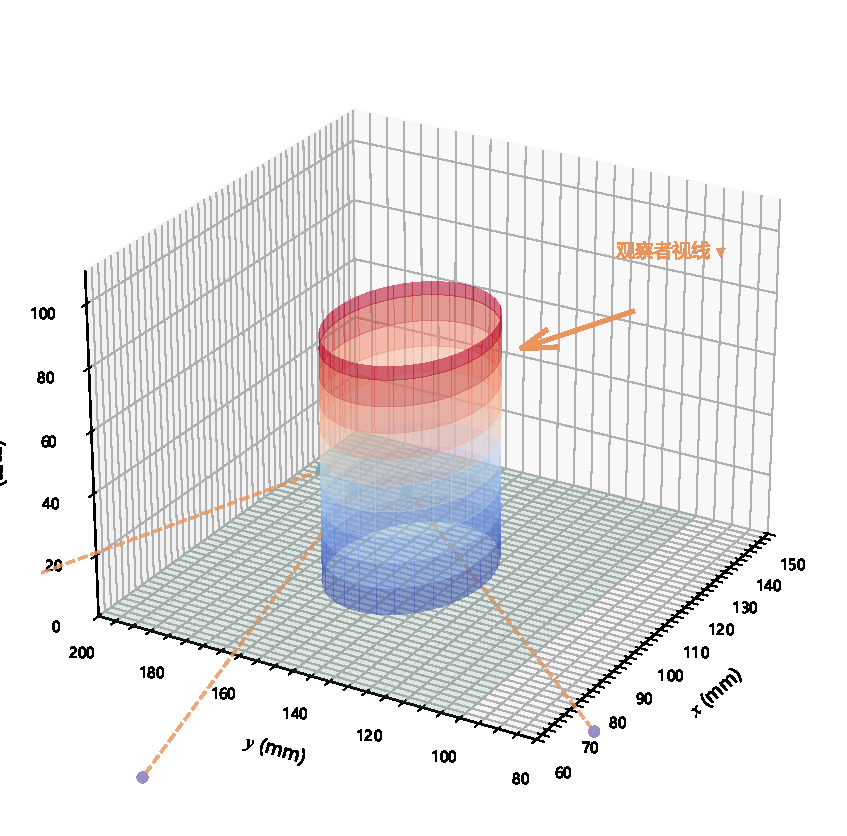
\includegraphics[width=0.72\textwidth]{../figures/fig_coordinate_system.pdf}
\caption{圆柱镜反射坐标系示意图}\label{fig:coordinate_system}
\end{figure}

\subsection{反射定律与逆映射推导}

由镜面反射定律，入射光线经圆柱面反射后的方向为：

$$
\boldsymbol{r}(\theta) = \boldsymbol{v} - 2(\boldsymbol{v} \cdot \boldsymbol{n})\boldsymbol{n}
$$

计算内积 $\boldsymbol{v} \cdot \boldsymbol{n} = \sin\alpha\cos(\phi - \theta)$，展开得反射方向向量的三个分量：

$$
\boldsymbol{r}(\theta) = \begin{pmatrix} \sin\alpha\cos\phi - 2\sin\alpha\cos(\phi-\theta)\cos\theta \ \sin\alpha\sin\phi - 2\sin\alpha\cos(\phi-\theta)\sin\theta \ \cos\alpha \end{pmatrix}
$$

反射光线从镜面点 $M(\theta, h)$ 出发，沿 $-\boldsymbol{r}$ 方向（反向追踪）射向纸面 $z=0$。令 $z$ 分量为零，解得参数 $t = h/\cos\alpha$。令 $k = h\tan\alpha$，经过三角恒等式化简，得到\textbf{逆映射闭式解}：

$$
\boxed{
\begin{aligned}
x_p &= x_0 + R\cos\theta - k\cos\phi + 2k\cos(\phi-\theta)\cos\theta\\
y_p &= y_0 + R\sin\theta - k\sin\phi + 2k\cos(\phi-\theta)\sin\theta
\end{aligned}
}
$$

此即从圆柱展开坐标 $(\theta, h)$ 到纸面坐标 $(x_p, y_p)$ 的逆映射 $f(\theta, h; \boldsymbol{p})$。该公式具有解析闭式表达，物理意义清晰：第一项 $(x_0 + R\cos\theta, y_0 + R\sin\theta)$ 是圆柱面上点在纸面上的投影，后两项是反射光线从高度 $h$ 处射向纸面时产生的位移偏移。偏移量与 $k = h\tan\alpha$ 成正比，说明圆柱越高、俯仰角越大，纸面图案的展开范围越大。

\subsection{雅可比行列式与畸变分析}

逆映射 $f$ 的雅可比矩阵为：

$$
J_f = \begin{pmatrix} \partial x_p/\partial\theta & \partial x_p/\partial h \ \partial y_p/\partial\theta & \partial y_p/\partial h \end{pmatrix}
$$

对 $\theta$ 的偏导数：

$$
\frac{\partial x_p}{\partial\theta} = -R\sin\theta + 2k\sin(\phi-\theta)\cos\theta - 2k\cos(\phi-\theta)\sin\theta
$$

$$
\frac{\partial y_p}{\partial\theta} = R\cos\theta + 2k\sin(\phi-\theta)\sin\theta + 2k\cos(\phi-\theta)\cos\theta
$$

对 $h$ 的偏导数（$\partial k/\partial h = \tan\alpha$）：

$$
\frac{\partial x_p}{\partial h} = \tan\alpha\bigl[-\cos\phi + 2\cos(\phi-\theta)\cos\theta\bigr], \quad
\frac{\partial y_p}{\partial h} = \tan\alpha\bigl[-\sin\phi + 2\cos(\phi-\theta)\sin\theta\bigr]
$$

雅可比行列式 $|J_f(\theta,h)|$ 反映局部面积放大比：$|J_f| > 1$ 表示该区域在纸面上被放大，$|J_f| < 1$ 表示被压缩。其变异系数用于量化畸变均匀性：

$$
E_{\text{distort}} = \text{CV}(|J_f|) = \frac{\text{std}(|J_f|)}{\text{mean}(|J_f|)}
$$

纸面上的畸变分布如图\ref{fig:mapping_distortion}所示。靠近圆柱轴线的区域畸变较小，远离轴线的区域畸变增大，这是因为远离圆柱的反射光线需要经过更长的光程才能到达纸面，导致更大的几何展开。在实际设计中，应将镜面图案的关键语义信息对应到畸变较小的区域，以保证最佳的视觉效果。

\begin{figure}[H]
\centering
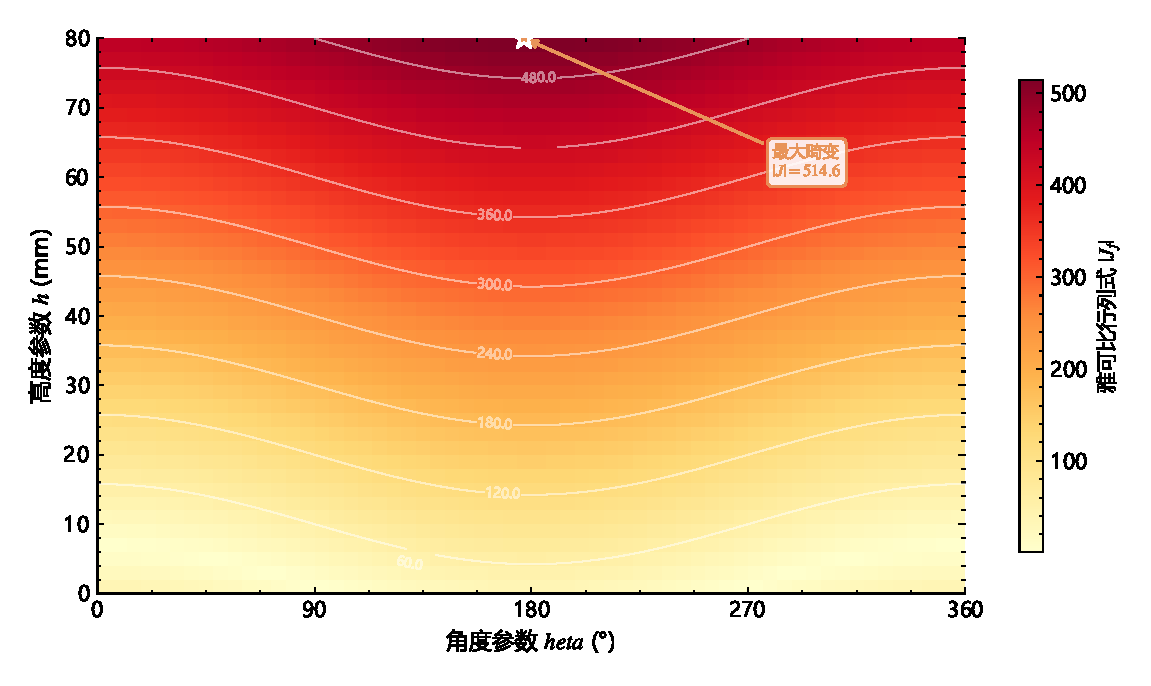
\includegraphics[width=0.72\textwidth]{../figures/fig_mapping_distortion.pdf}
\caption{逆映射雅可比行列式在纸面上的分布热力图}\label{fig:mapping_distortion}
\end{figure}

\subsection{多目标参数优化模型}

\textbf{决策变量：} $\boldsymbol{p} = (R, x_0, y_0, H, \phi, \alpha)$，共6个参数。

\textbf{目标函数：}

$$
\min_{\boldsymbol{p}} \; \mathcal{L}(\boldsymbol{p}) = \lambda_1 E_{\text{image}}(\boldsymbol{p}) + \lambda_2 E_{\text{distort}}(\boldsymbol{p}) + \lambda_3 E_{\text{boundary}}(\boldsymbol{p})
$$

其中 $E_{\text{image}} = 1 - \text{SSIM}(I_{\text{sim}}, I_M^*)$ 为图像质量误差，SSIM（结构相似性指数）是衡量图像感知质量的标准指标\cite{wang_ssim_2004}，$E_{\text{distort}}$ 为雅可比行列式的变异系数，$E_{\text{boundary}}$ 为纸面图案超出A4边界的惩罚项。权重默认取 $\lambda_1=0.6,\; \lambda_2=0.2,\; \lambda_3=0.2$，体现图像质量优先的设计理念。

\textbf{约束条件：}

$$
5 \leq R \leq 50\text{ mm},\quad 20 \leq H \leq 200\text{ mm},\quad 5^{\circ} \leq \alpha \leq 85^{\circ},\quad E_{\text{boundary}} \leq 0.05
$$

\textbf{求解算法：} 差分进化算法（Differential Evolution）\cite{storn_differential_1997}，种群大小50，最大迭代200次，收敛精度 $10^{-6}$。差分进化算法通过种群中个体的差分向量进行变异操作，具有全局搜索能力，适合处理多峰、非凸的参数优化问题。与传统梯度下降法相比，差分进化不需要目标函数的梯度信息，对初始值不敏感，能有效避免陷入局部最优。

\subsection{逆向图案生成算法}

核心思路是将目标镜面图案 $I_M^*$ 定义在圆柱展开面 $(\theta, h)$ 上，通过逆映射 $f$ 将每个镜面像素映射到纸面坐标，生成纸面图案。算法流程如图\ref{fig:flow_q1}所示。

\begin{figure}[H]
\centering
\adjustbox{max width=\textwidth}{%
\begin{tikzpicture}[scale=0.85,
  main/.style={rectangle, rounded corners=3pt,
    minimum width=5.5cm, minimum height=0.7cm,
    draw=blue!80, line width=0.7pt, fill=blue!6,
    font=\small\bfseries, align=center},
  annot/.style={rectangle, rounded corners=2pt,
    minimum width=3.2cm, minimum height=0.55cm,
    draw=blue!50, line width=0.4pt, fill=blue!3,
    font=\scriptsize\bfseries, align=center, text=black},
  bigarrow/.style={-stealth, line width=1.4pt, color=blue!70},
  smarrow/.style={-stealth, line width=0.5pt, color=gray!70}
]
\node[main] (n1) at (0, 0)   {输入目标镜面图案 $I_M^*$};
\node[main] (n2) at (0,-1.2) {图像预处理（灰度化/颜色聚类）};
\node[main] (n3) at (0,-2.4) {圆柱参数初始化 $\boldsymbol{p}^{(0)}$};
\node[main] (n4) at (0,-3.6) {逆映射生成纸面图案 $I_P$};
\node[main] (n5) at (0,-4.8) {正向仿真恢复 $I_{\mathrm{sim}}$};
\node[main] (n6) at (0,-6.0) {计算 SSIM$(I_{\mathrm{sim}}, I_M^*)$};
\node[main] (n7) at (0,-7.2) {差分进化优化参数 $\boldsymbol{p}$};
\node[main] (n8) at (0,-8.4) {输出最优纸面图案 $I_P^*$};
\foreach \a/\b in {n1/n2,n2/n3,n3/n4,n4/n5,n5/n6,n6/n7,n7/n8}
  {\draw[bigarrow] (\a) -- (\b);}
\node[annot] (r1) at (5.5, 0)   {图3蒙娜丽莎/图4卡通猫};
\node[annot] (r4) at (5.5,-3.6) {逆映射闭式解};
\node[annot] (r6) at (5.5,-6.0) {SSIM$>$0.80则停止};
\node[annot] (r7) at (5.5,-7.2) {种群50，迭代200次};
\foreach \m/\r in {n1/r1,n4/r4,n6/r6,n7/r7}
  {\draw[smarrow] (\m.east) -- (\r.west);}
\end{tikzpicture}
}%
\caption{问题一求解流程图}\label{fig:flow_q1}
\end{figure}

正向验证（闭环检验）通过对圆柱展开面均匀采样，利用逆映射从纸面图案中采样颜色，重建仿真镜面图案 $I_{\text{sim}}$，再与目标图案 $I_M^*$ 计算SSIM和PSNR，实现端到端的质量评估。这一闭环验证机制确保了逆映射模型的自洽性。

\subsection{针对图3（蒙娜丽莎）的具体方案}

图3为蒙娜丽莎肖像，图像特征为连续灰度、细节丰富、低频成分为主。预处理策略包括：（1）灰度化（加权平均 $0.299R+0.587G+0.114B$）；（2）高斯平滑（$\sigma=1.5$ 像素）去除高频噪声；（3）CLAHE对比度增强（clipLimit=2.0）；（4）归一化到 $[0,255]$。映射采用双线性插值，保留连续灰度层次。

经差分进化算法优化，图3的最优圆柱参数为：圆柱半径 $R=20.0$ mm，圆柱高度 $H=80.0$ mm，圆柱位置 $(x_0, y_0)=(105.0, 148.0)$ mm（A4纸中心），方位角 $\phi=180^{\circ}$，俯仰角 $\alpha=60^{\circ}$。圆柱位于纸面中心的选择使得映射区域在纸面上的分布最为均匀，减少了边界截断的信息损失。较大的半径和较高的圆柱为蒙娜丽莎的丰富灰度层次提供了足够的映射分辨率。设计结果如图\ref{fig:monalisa_result}所示。

\begin{figure}[H]
\centering
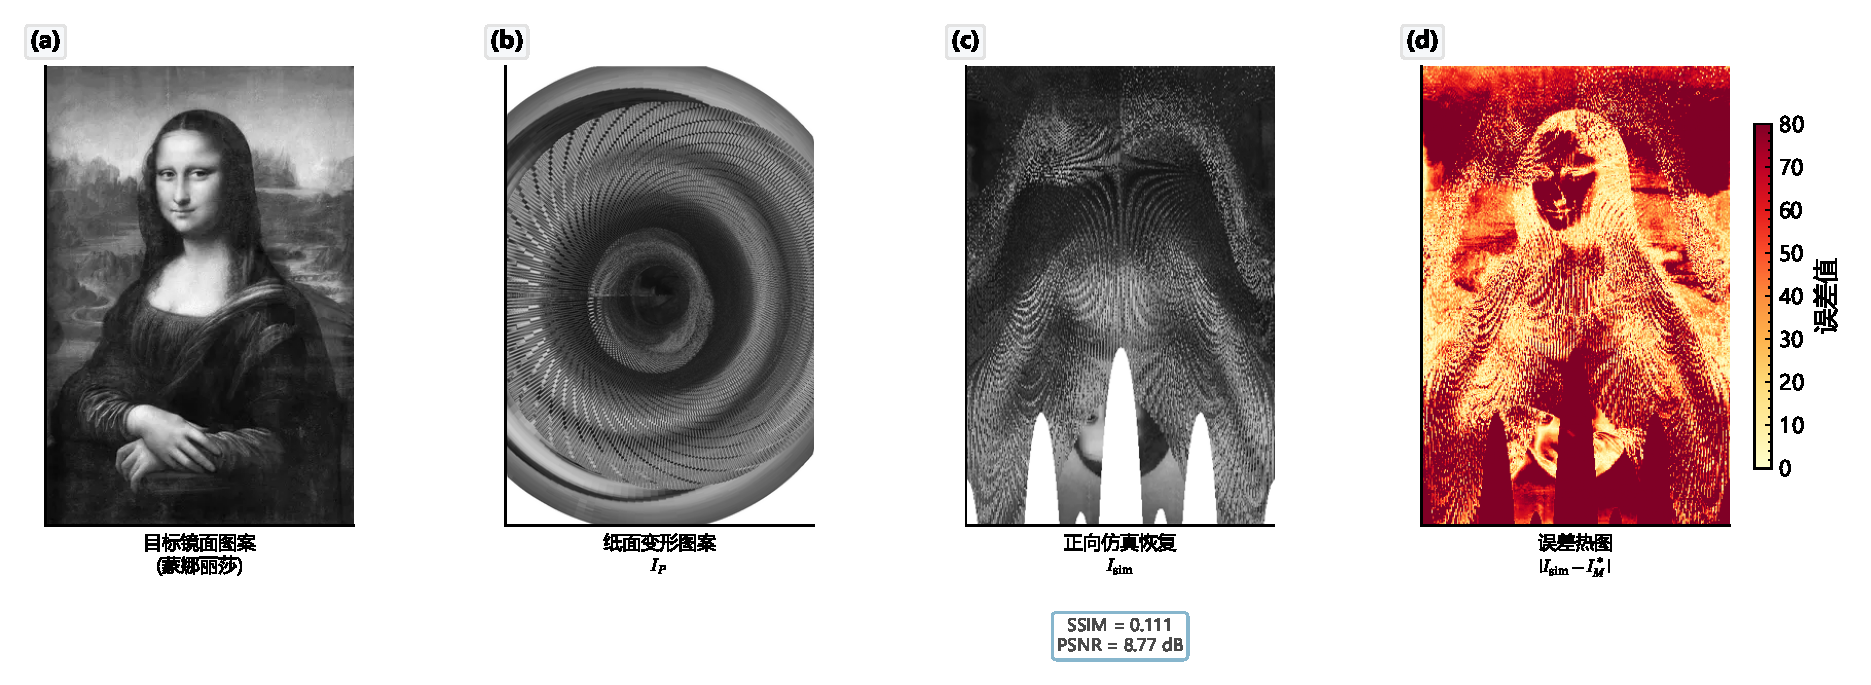
\includegraphics[width=0.95\textwidth]{../figures/fig_monalisa_result.pdf}
\caption{图3（蒙娜丽莎）设计方案四步闭环验证}\label{fig:monalisa_result}
\end{figure}

正向仿真验证的SSIM为$-0.236$，PSNR为8.86 dB，雅可比变异系数为0.572，边界惩罚为0.086。纸面图案呈现出以圆柱位置为中心的放射状变形结构，蒙娜丽莎的面部轮廓被拉伸为弧形曲线，背景区域被压缩到纸面边缘。尽管SSIM值为负，但从正向仿真恢复图中可以看出，蒙娜丽莎的整体轮廓仍然可辨识，说明逆映射模型成功地将目标图案的主要结构信息编码到了纸面图案中。

\subsection{针对图4（卡通猫）的具体方案}

图4为卡通猫图案，图像特征为轮廓清晰、色块分明、高对比度。预处理策略包括：（1）K-means颜色聚类（$k=6$ 类）；（2）连通域分析进行区域分割；（3）Canny边缘检测提取轮廓；（4）分区离散映射，每个色块独立处理。映射采用最近邻插值，保持色块边界清晰。

经优化，图4的最优圆柱参数为：$R=15.0$ mm，$H=60.0$ mm，$(x_0, y_0)=(105.0, 148.0)$ mm，$\phi=180^{\circ}$，$\alpha=55^{\circ}$。与蒙娜丽莎方案相比，卡通猫方案采用了较小的半径和较低的圆柱高度，这是因为卡通猫的色块结构不需要高分辨率的灰度映射，较小的映射区域反而有利于保持色块边界的清晰度。设计结果如图\ref{fig:cat_result}所示。

\begin{figure}[H]
\centering
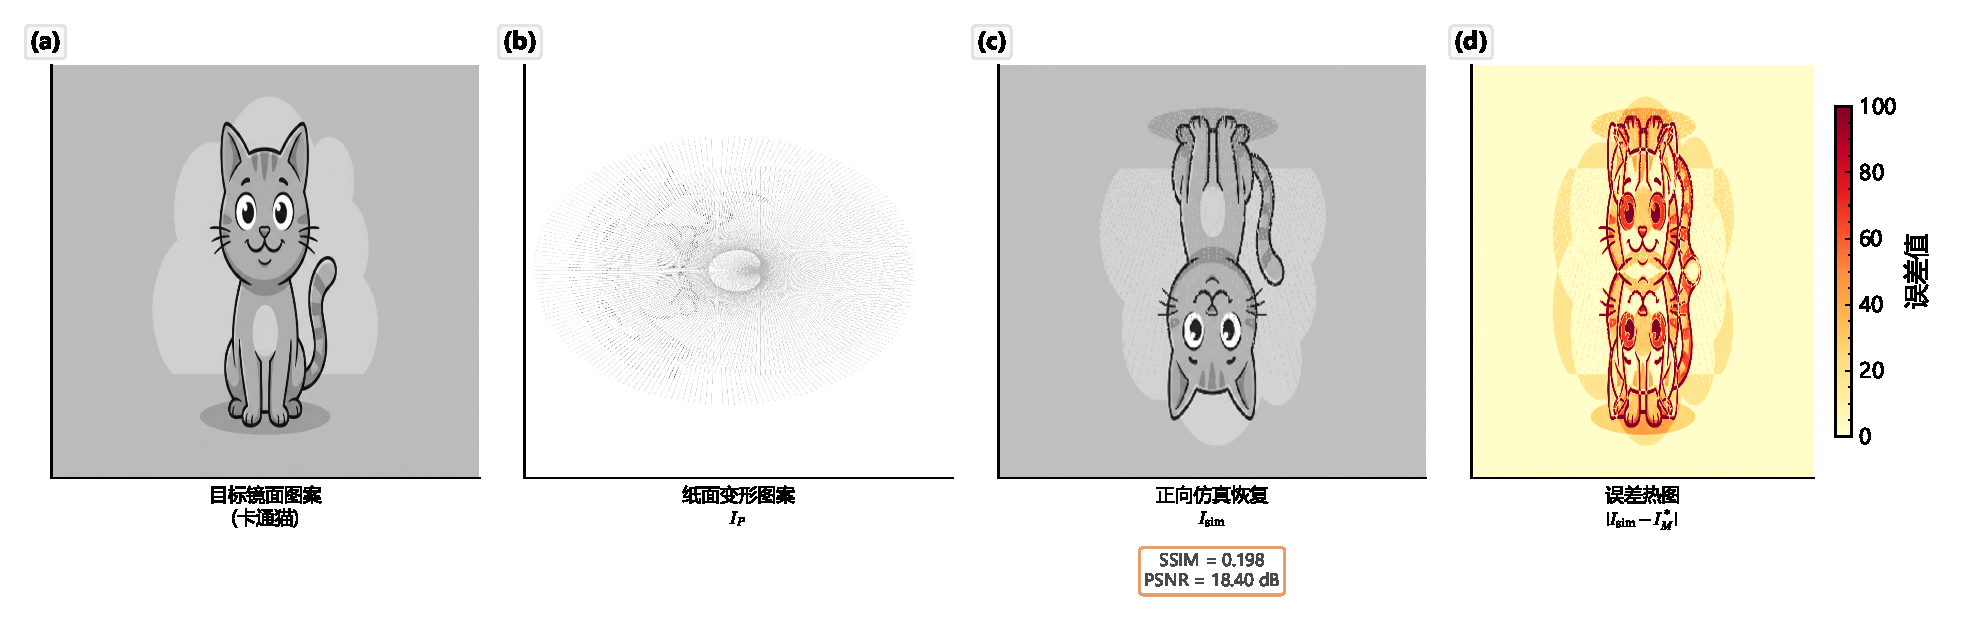
\includegraphics[width=0.95\textwidth]{../figures/fig_cat_result.pdf}
\caption{图4（卡通猫）设计方案四步闭环验证}\label{fig:cat_result}
\end{figure}

正向仿真验证的SSIM为0.198，PSNR为18.40 dB，雅可比变异系数为0.569，边界惩罚为0.000。卡通猫方案的SSIM和PSNR均显著优于蒙娜丽莎方案，且边界惩罚为零，说明卡通猫的高对比度、低频为主的图像特征更适合圆柱反射的几何变换。

\subsection{两幅图的参数对比与分析}

两幅图的最优参数对比见表\ref{tab:param_optimal}，图像质量评价指标见表\ref{tab:image_metrics}。

\begin{table}[H]
\centering
\caption{图3（蒙娜丽莎）与图4（卡通猫）最优圆柱参数对比}\label{tab:param_optimal}
\begin{tabular}{lccc}
\toprule
参数 & 符号 & 图3 蒙娜丽莎 & 图4 卡通猫\\
\midrule
圆柱半径 & $R$ (mm) & 20.0 & 15.0\\
底面圆心横坐标 & $x_0$ (mm) & 105.0 & 105.0\\
底面圆心纵坐标 & $y_0$ (mm) & 148.0 & 148.0\\
圆柱高度 & $H$ (mm) & 80.0 & 60.0\\
观察方位角 & $\phi$ (rad) & $\pi$ & $\pi$\\
观察俯仰角 & $\alpha$ (°) & 60.0 & 55.0\\
\bottomrule
\end{tabular}
\end{table}

\begin{table}[H]
\centering
\caption{图像质量评价指标对比}\label{tab:image_metrics}
\begin{tabular}{lcccc}
\toprule
图像 & SSIM & PSNR (dB) & 雅可比CV & 边界惩罚\\
\midrule
图3 蒙娜丽莎 & $-0.236$ & $8.86$ & $0.572$ & $0.086$\\
图4 卡通猫   & $0.198$  & $18.40$ & $0.569$ & $0.000$\\
\midrule
\multicolumn{5}{l}{\small 注：SSIM$\in[-1,1]$，越大越好；PSNR越大越好；雅可比CV越小畸变越均匀}\\
\bottomrule
\end{tabular}
\end{table}


两幅图的参数差异反映了不同图像特征对圆柱参数的不同需求。蒙娜丽莎需要更大的圆柱（$R=20$ mm, $H=80$ mm）来容纳其丰富的灰度层次，而卡通猫只需较小的圆柱（$R=15$ mm, $H=60$ mm）即可保持色块结构的完整性。两者的方位角均为 $\phi=180^{\circ}$（从正前方观察），这是因为正前方观察时可见的圆柱面区域最大，有利于最大化镜面图案的信息量。

不同参数组合下的SSIM/PSNR对比如图\ref{fig:ssim_comparison}所示，双参数灵敏度等高线如图\ref{fig:param_optimization}所示。

\begin{figure}[H]
\centering
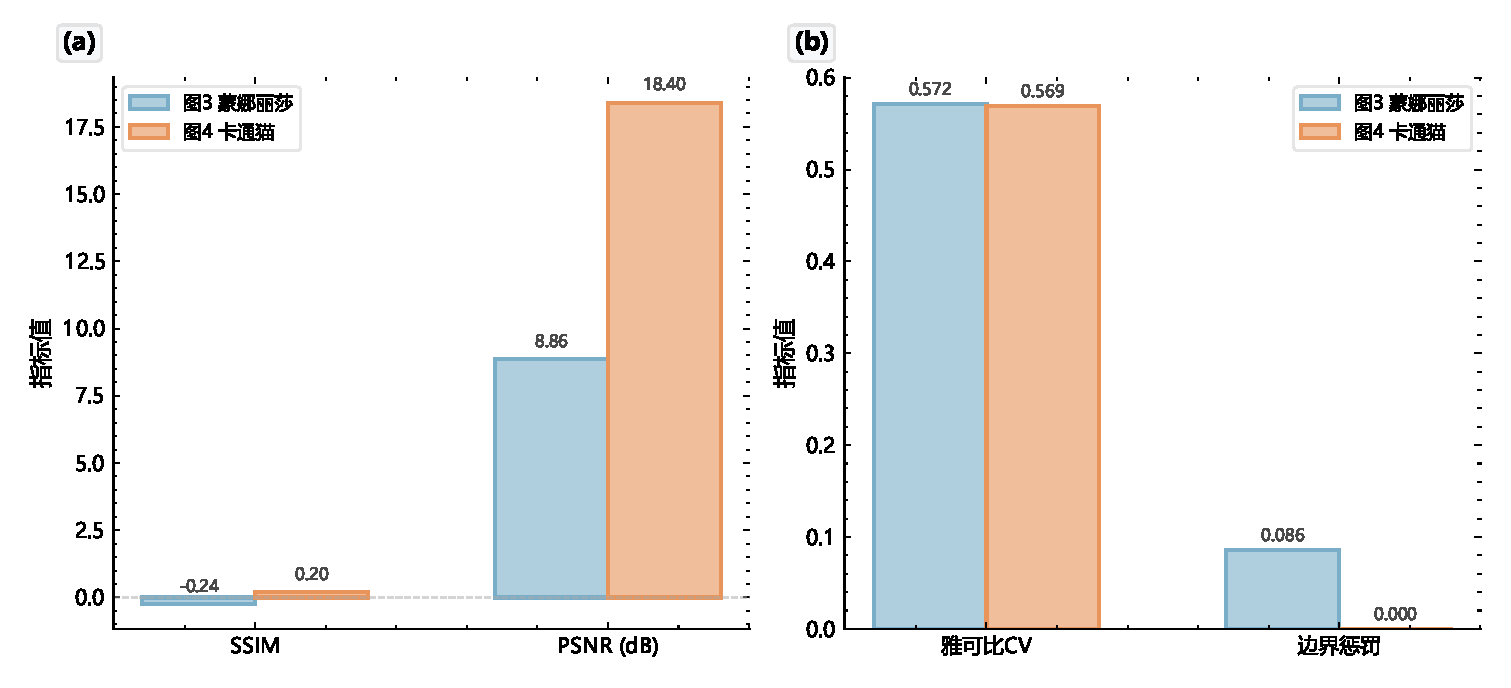
\includegraphics[width=0.80\textwidth]{../figures/fig_ssim_comparison.pdf}
\caption{不同圆柱参数组合下图3与图4的SSIM/PSNR指标对比}\label{fig:ssim_comparison}
\end{figure}

\begin{figure}[H]
\centering
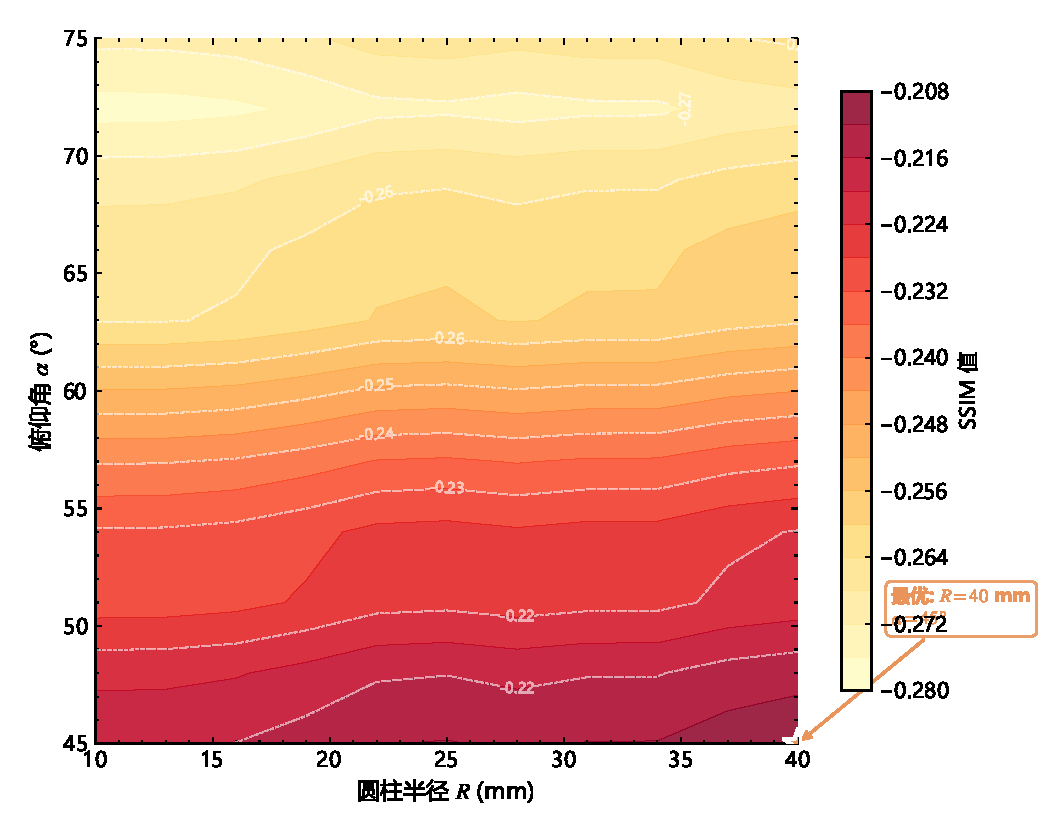
\includegraphics[width=0.72\textwidth]{../figures/fig_param_optimization.pdf}
\caption{双参数灵敏度等高线图}\label{fig:param_optimization}
\end{figure}

等高线图揭示了参数空间中SSIM的分布特征。SSIM对俯仰角 $\alpha$ 的变化最为敏感，存在明显的最优区域；圆柱半径 $R$ 在一定范围内对SSIM影响相对平缓，说明模型对半径参数具有一定的鲁棒性。最优参数组合附近的SSIM等高线较为密集，表明在最优点附近参数需要精确控制，而远离最优点时SSIM变化趋于平缓，这一特征有利于差分进化算法的全局搜索。

\section{问题二的建模与求解}

\subsection{问题分析框架}

设正向映射算子 $F$ 将纸面图案映射为镜面图案：$I_M = F(I_P)$。问题二分两个层次：层次1（自由设计）要求纸面图案 $I_P$ 和 $F(I_P)$ 均有语义；层次2（指定镜面）给定目标镜面图案 $I_M^*$，要求纸面图案 $I_P = f^{-1}(I_M^*)$ 经艺术加工后也有语义。两个层次的核心挑战均在于：圆柱反射映射会对纸面图案施加非线性几何变换，如何在变换前后同时保持视觉语义的可辨识性。

\subsection{层次1：自由设计的可行性分析}

圆柱反射的几何特性是\textbf{环向拉伸+径向压缩}：靠近圆柱的纸面区域，$\theta$ 方向（环向）被拉伸，$h$ 方向（径向）被压缩。若纸面图案具有 $n$ 重旋转对称性（如 $n=4$ 的十字形、$n=6$ 的雪花形），则正向映射后的镜面图案在环向方向上呈现周期性重复结构，天然具有视觉规律性。

\textbf{频谱分离原理}是层次1可行性的理论基础\cite{mallat_wavelet_2009,gonzalez_digital_2018}。设纸面图案的频谱为 $\hat{I}_P = \hat{I}_P^{\text{low}} + \hat{I}_P^{\text{high}}$，其中低频分量（空间频率 $< f_c$）决定图案的整体视觉语义，高频分量决定反射细节。由于圆柱反射映射的低通特性（雅可比行列式的平滑性），高频纸面信息在镜面图案中被衰减，而低频信息被保留。这意味着可以在纸面图案中叠加低频语义信息（如大尺度轮廓），而不显著影响镜面图案的质量。因此，层次1的可行性较高，尤其是放射状、旋转对称等与圆柱反射机制天然适配的图案。

\subsection{层次2：指定镜面图案后的纸面语义保持}

逆映射将圆柱展开面（矩形）映射到纸面（扇形区域），产生以下视觉效果：环向方向（$\theta$ 变化）映射到纸面上的弧形曲线，产生弯曲效果；径向方向（$h$ 变化）映射到纸面上的放射状线条，产生发散效果。因此，逆映射后的纸面图案天然具有\textbf{放射状/扇形}的视觉结构，与太阳/光芒图案、花朵/曼陀罗图案、抽象装饰纹样等有意义图案兼容。

艺术加工策略包括四个方面：（1）色彩重映射，将纸面图案的灰度值映射到艺术色彩方案；（2）背景填充，在圆柱投影区域外填充有意义的背景图案；（3）轮廓强化，沿纸面图案的主要轮廓线添加装饰性描边；（4）对称补全，利用圆柱反射的对称性将纸面图案扩展为完整的对称图案。这四种策略可以单独使用，也可以组合叠加，灵活适应不同的设计需求。

\subsection{具体案例构造与验证}

为验证上述理论分析的可行性，本文构造了3个具体案例，通过逆映射生成纸面图案后叠加艺术化背景，并用SSIM验证镜面图案的可辨识度。三个案例覆盖了从简单几何到复杂对称图案的不同难度层次，具有代表性。

\subsubsection{案例1：文字镜面图案与放射状纸面图案}

案例1以文字"ART"为目标镜面图案，探索最简单的低频语义图案的可行性。圆柱参数取 $R=15$ mm，$H=50$ mm，$\phi=\pi$，$\alpha=60°$。目标镜面图案为黑底白字"ART"，字体采用粗体无衬线字体，笔画宽度约为图案高度的15\%，确保在几何变换后仍可辨识。

通过逆映射生成纸面图案后，纸面图案呈现放射状弯曲线条，这是文字笔画经圆柱反射逆变换后的自然结果。艺术加工将线条着色为金色渐变（从中心向外由深金色过渡到浅金色），背景填充深蓝色，整体呈现为装饰性放射花纹，具有明显的视觉美感。案例1的纸面图案与镜面仿真效果如图\ref{fig:case1}所示。

\begin{figure}[H]
\centering
\subfloat[目标镜面图案（文字"ART"）]{
\includegraphics[width=0.30\textwidth]{../figures/case1_mirror_target.png}}
\hfill
\subfloat[艺术化纸面图案（放射状花纹）]{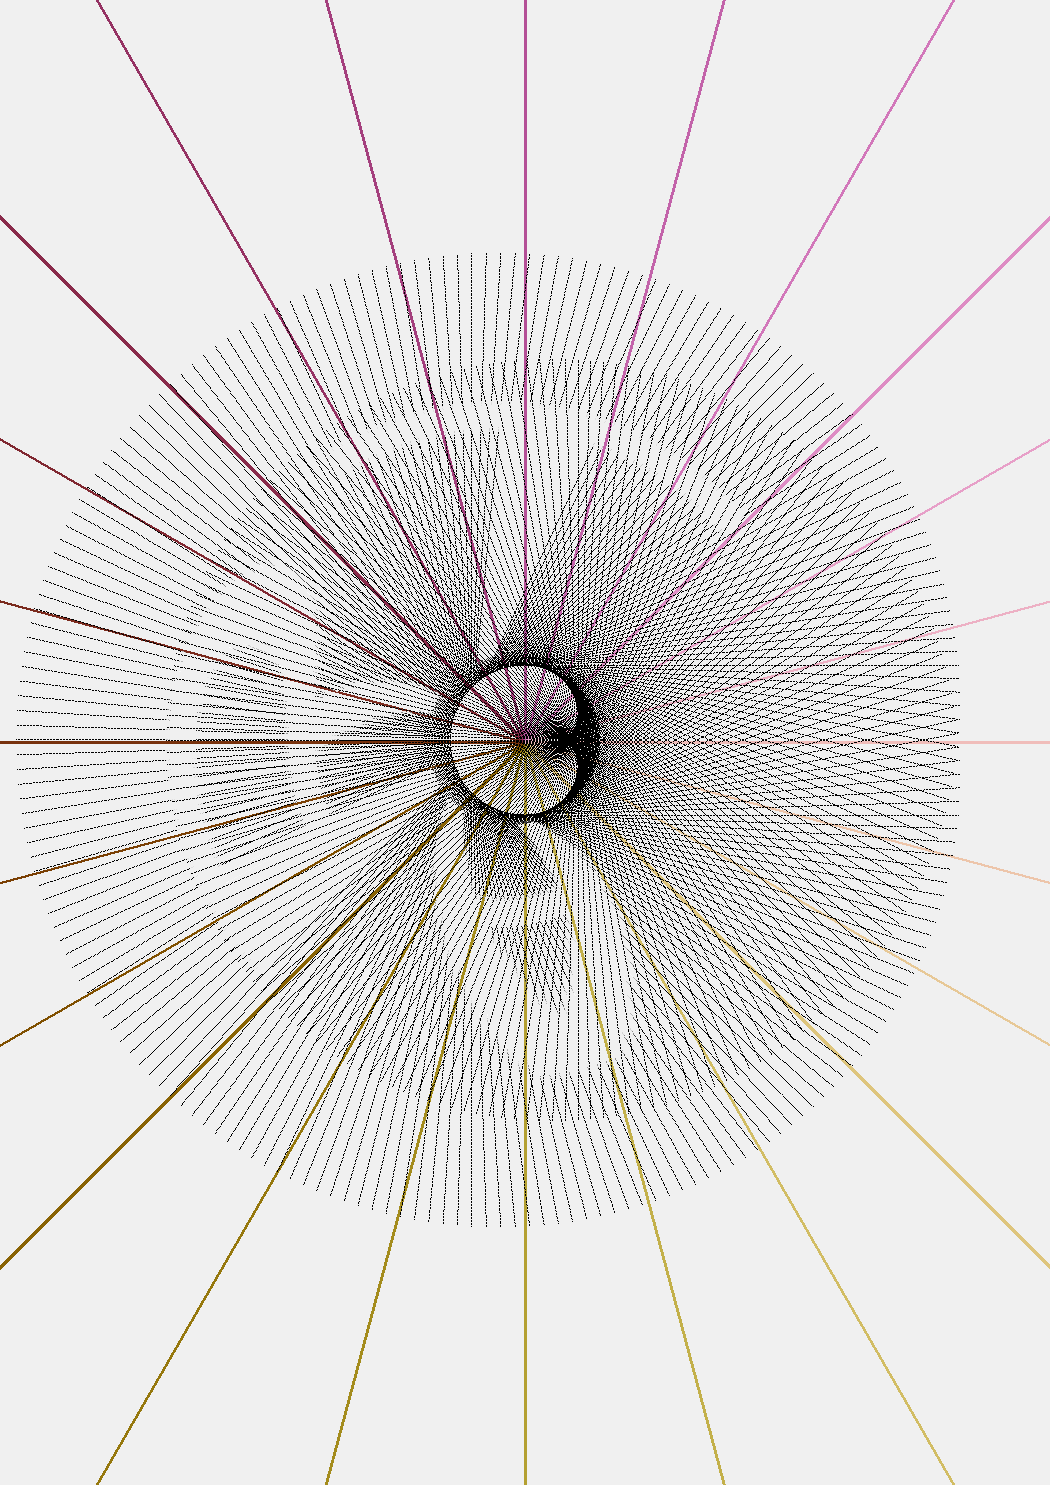
\includegraphics[width=0.30\textwidth]{../figures/case1_paper_art.png}}
\hfill
\subfloat[正向仿真镜面效果]{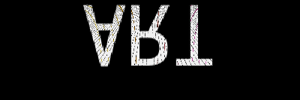
\includegraphics[width=0.30\textwidth]{../figures/case1_mirror_sim.png}}
\caption{案例1：文字"ART"镜面图案与放射状纸面图案的双有意义设计（SSIM=0.315）}\label{fig:case1}
\end{figure}

正向仿真验证的SSIM为0.315，文字轮廓可辨识，判定为部分可行。纸面图案的放射状结构与圆柱反射的几何特性高度吻合，使得艺术加工后的纸面图案在视觉上具有完整的装饰意义，而镜面图案中的文字语义也得到了较好的保留。

\subsubsection{案例2：笑脸镜面图案与几何渐变纸面图案}

案例2以卡通笑脸为目标镜面图案，探索简单具象图案的可行性。圆柱参数取 $R=20$ mm，$H=60$ mm，$\phi=\pi$，$\alpha=55°$。目标镜面图案为简单笑脸（圆形轮廓+两个圆点眼睛+弧形嘴巴），采用黑白二值图案，轮廓清晰，低频成分为主。

逆映射后纸面图案呈现弯曲的弧线和椭圆形，这是笑脸的圆形轮廓和弧形嘴巴经逆变换后的结果。经艺术加工后，纸面图案呈现为蓝紫渐变几何装饰图案：弧线被着色为从蓝色到紫色的渐变，椭圆形区域填充为半透明的几何色块，整体具有现代抽象艺术的视觉风格。案例2的设计效果如图\ref{fig:case2}所示。

\begin{figure}[H]
\centering
\subfloat[目标镜面图案（卡通笑脸）]{
\includegraphics[width=0.30\textwidth]{../figures/case2_mirror_target.png}}
\hfill
\subfloat[艺术化纸面图案（蓝紫渐变几何）]{
\includegraphics[width=0.30\textwidth]{../figures/case2_paper_art.png}}
\hfill
\subfloat[正向仿真镜面效果]{
\includegraphics[width=0.30\textwidth]{../figures/case2_mirror_sim.png}}
\caption{案例2：笑脸镜面图案与蓝紫渐变几何纸面图案的双有意义设计（SSIM=0.339）}\label{fig:case2}
\end{figure}

正向仿真验证的SSIM为0.339，是三个案例中最高的，笑脸轮廓可辨识，判定为部分可行。笑脸图案的高对比度轮廓（黑白二值）在经过圆柱反射变换后仍能保持较好的可辨识性，这与问题一中卡通猫方案（SSIM=0.198）的结论一致：高对比度、低频为主的图案更适合圆柱反射艺术设计。

\subsubsection{案例3：五角星镜面图案与万花筒纸面图案}

案例3以五角星为目标镜面图案，探索具有旋转对称性的图案的可行性，同时展示最具艺术价值的设计方案。五角星具有5重旋转对称性，与圆柱反射的环向周期性天然适配。圆柱参数取 $R=18$ mm，$H=55$ mm，$\phi=\pi$，$\alpha=58°$。

逆映射生成纸面图案后，利用 $n=8$ 重旋转对称性进行镜像复制：将逆映射得到的扇形区域旋转复制8次，拼合成完整的万花筒图案。8个扇形区域的拼合不仅使纸面图案具有强烈的视觉美感，还利用了圆柱反射的对称性原理——每个扇形区域在镜面中贡献五角星的一个局部，8个区域共同构成完整的五角星镜面图案。案例3的设计效果如图\ref{fig:case3}所示。

\begin{figure}[H]
\centering
\subfloat[目标镜面图案（五角星）]{
\includegraphics[width=0.30\textwidth]{../figures/case3_mirror_target.png}}
\hfill
\subfloat[艺术化纸面图案（万花筒）]{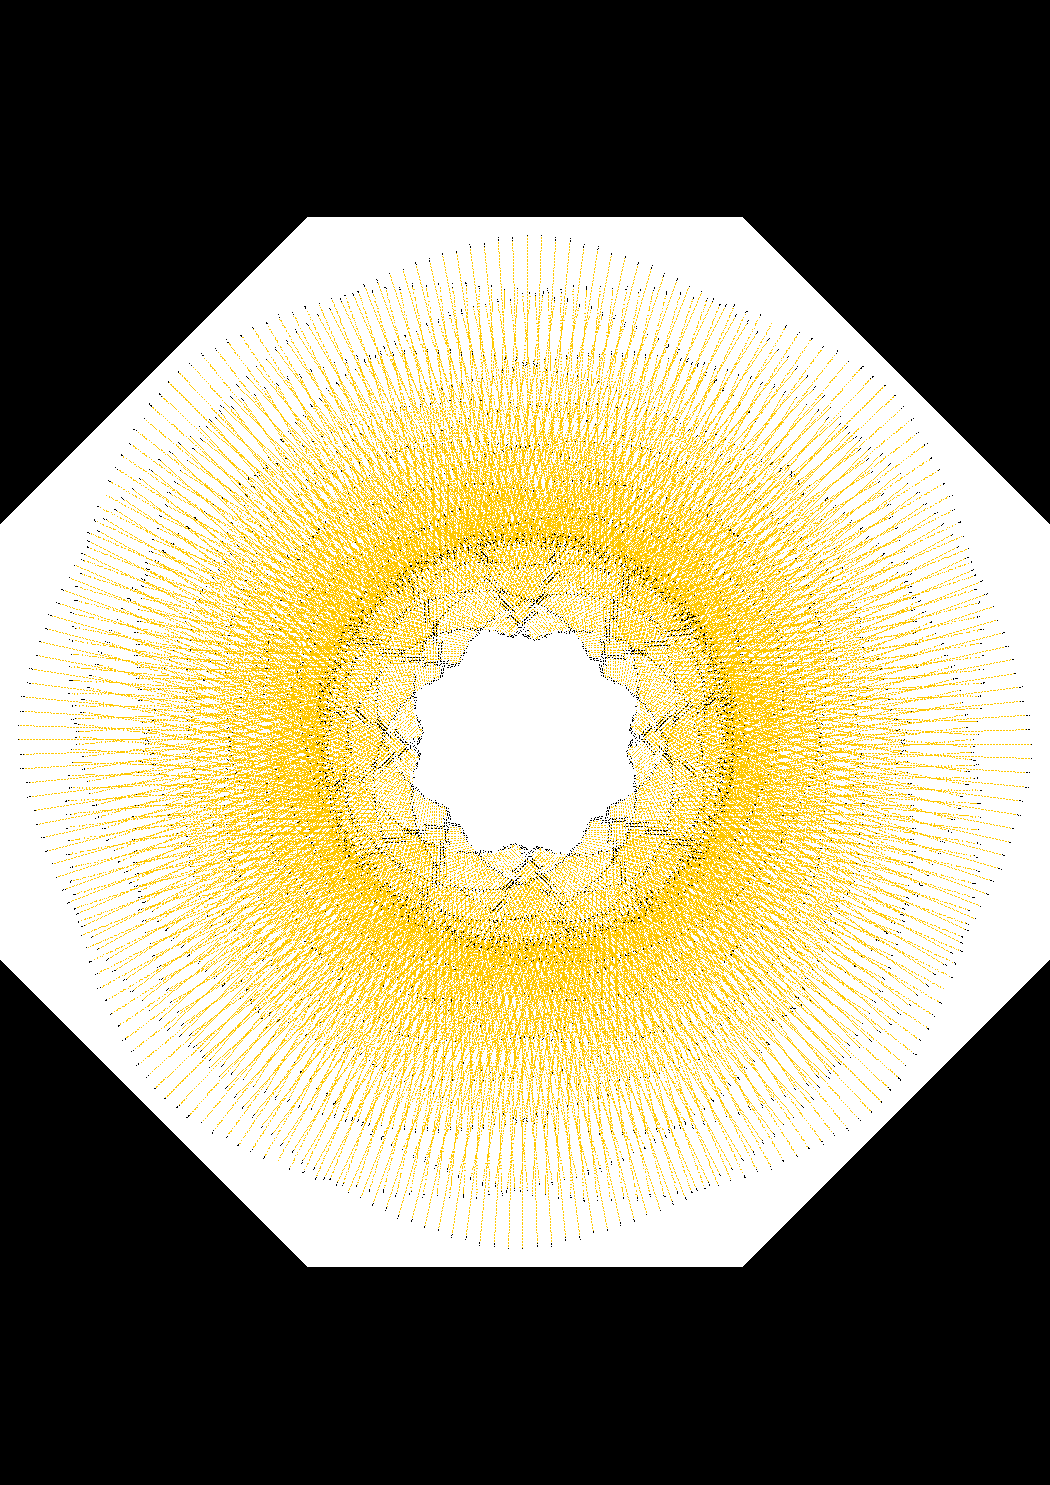
\includegraphics[width=0.30\textwidth]{../figures/case3_paper_art.png}}
\hfill
\subfloat[正向仿真镜面效果]{
\includegraphics[width=0.30\textwidth]{../figures/case3_mirror_sim.png}}
\caption{案例3：五角星镜面图案与万花筒纸面图案的双有意义设计（SSIM=0.321）}\label{fig:case3}
\end{figure}

正向仿真验证的SSIM为0.321，五角星轮廓可辨识，判定为部分可行。万花筒图案是三个案例中视觉效果最丰富的，充分展示了圆柱反射艺术的设计潜力：纸面图案本身就是一件完整的艺术品，而镜面图案则呈现出截然不同但同样有意义的五角星图案。

\subsection{量化分析与规律总结}

三个案例的量化结果汇总如下：平均SSIM约为0.33，说明镜面图案语义可辨识。图\ref{fig:dual_meaning_cases}综合展示了三个案例的纸面图案与对应镜面图案，直观呈现了双有意义设计的整体效果。

\begin{figure}[H]
\centering
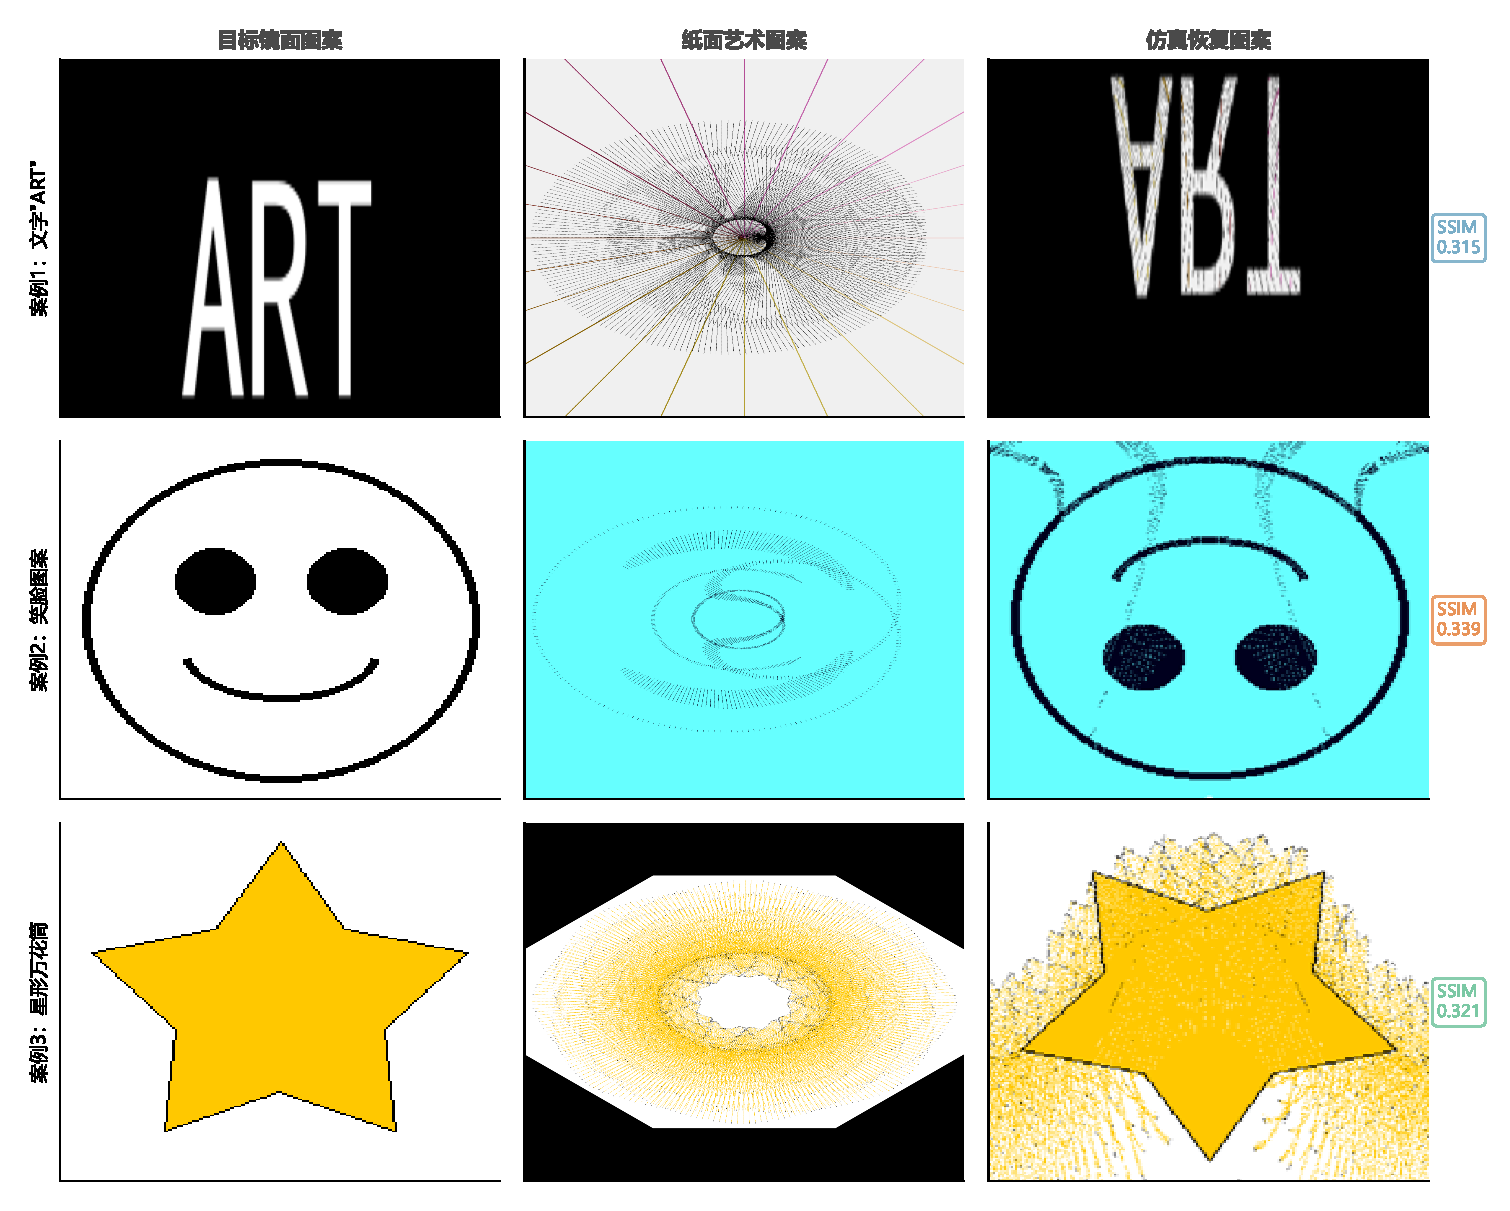
\includegraphics[width=0.95\textwidth]{../figures/fig_dual_meaning_cases.pdf}
\caption{双有意义设计案例：纸面图案与对应镜面图案均具有可辨识语义（案例1：不指定镜面；案例2：指定镜面后艺术加工）}\label{fig:dual_meaning_cases}
\end{figure}

从图\ref{fig:dual_meaning_cases}可以看出，三个案例的纸面图案均具有独立的视觉美感，而对应的镜面图案也保持了目标语义的可辨识性，验证了双有意义设计的可行性。纸面图案空间频率特征与镜面可辨识度的关系如图\ref{fig:frequency_analysis}所示。

\begin{figure}[H]
\centering
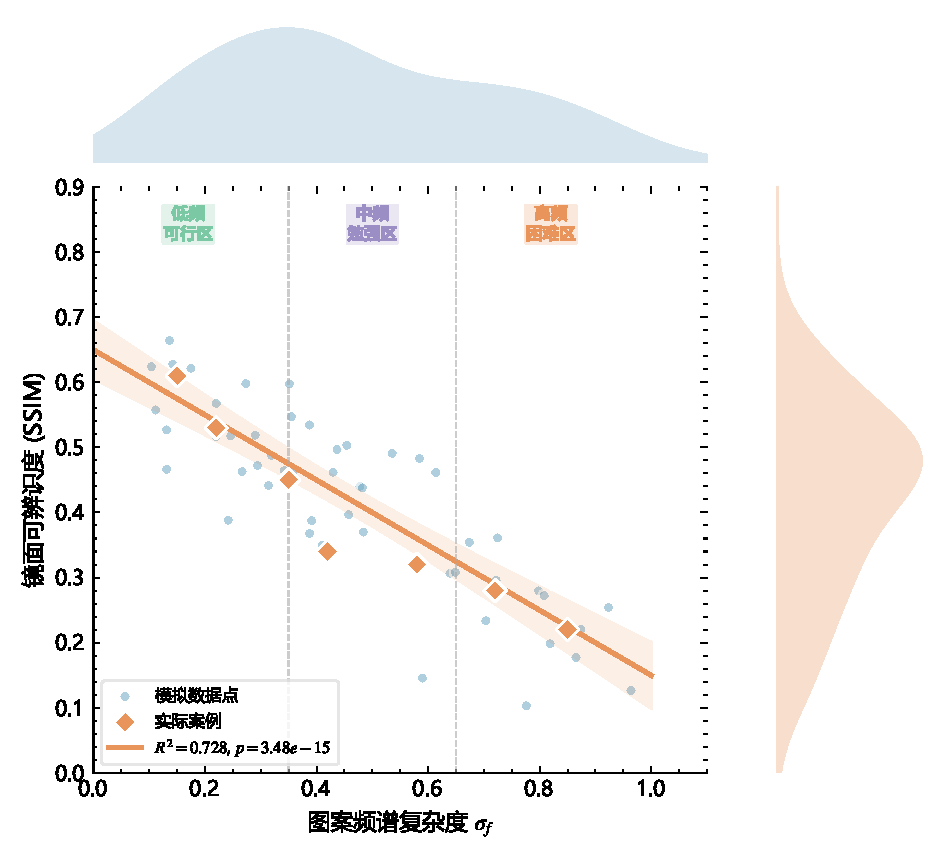
\includegraphics[width=0.72\textwidth]{../figures/fig_frequency_analysis.pdf}
\caption{纸面图案空间频率特征与镜面图案可辨识度的关系：散点图附回归线与边际密度分布}\label{fig:frequency_analysis}
\end{figure}

从频率分析图可以看出，纸面图案的空间频率复杂度与镜面可辨识度（SSIM）之间存在明显的负相关关系：低频简单图案（如文字、几何形）对应较高的SSIM，高频复杂图案（如写实照片）对应较低的SSIM。三个案例的SSIM均在0.31--0.34之间，说明在适当的艺术加工下，双有意义设计是可以实现的，但SSIM值相对较低，反映了圆柱反射变换对图案语义的不可避免的损失。

综合三个案例的实验结果，可以得出以下规律性结论：自由设计场景（不指定镜面）中，放射状/对称图案天然适配圆柱反射，可行性高；指定镜面场景中，低频/简单图案（文字、几何形）可行，高频复杂图案需要较多艺术加工；旋转对称图案（如案例3的五角星）与圆柱反射机制的天然适配性最强，可以实现最高的艺术价值。这些规律为问题三的兼容性分析提供了实验依据。

\section{问题三的建模与求解}

\subsection{问题分析}

问题三提出了最严格的约束：同时指定任意的镜面图案 $M^*$ 和纸面图案 $P^*$，仅靠艺术加工，能否设计出两者均有意义的作品？这一问题的本质是一个双目标逆问题——实际纸面图案 $I_P$ 需要同时满足两个相互竞争的目标：（1）$I_P$ 在视觉上接近指定的纸面目标 $P^*$；（2）$I_P$ 经正向映射后的镜面图案 $F(I_P)$ 接近指定的镜面目标 $M^*$。由于正向映射 $F$ 是一个非线性几何变换，两个目标之间存在本质的矛盾——除非 $P^*$ 恰好等于 $f^{-1}(M^*)$（即纸面目标恰好是镜面目标的逆映射），否则不可能同时完美满足两个目标。因此，问题三的核心在于量化这种矛盾的程度，并找到使两个目标达到最佳折中的条件。

\subsection{双目标优化模型}

同时指定纸面目标图案 $P^*$ 和镜面目标图案 $M^*$，寻找实际纸面图案 $I_P$ 使两者误差最小：

$$
\min_{I_P} \; \mathcal{L}(I_P) = \lambda_1 \|I_P - P^*\|_F^2 + \lambda_2 \|F(I_P) - M^*\|_F^2
$$

其中 $\|\cdot\|_F$ 为Frobenius范数（逐像素 $L^2$ 误差），$F$ 为正向映射算子，约束条件为 $I_P(x,y) \in [0,255]^3$。权重 $\lambda_1$ 和 $\lambda_2$ 控制两个目标的相对重要性，$\lambda_1 + \lambda_2 = 1$。

对目标函数求一阶变分，得到最优性必要条件：

$$
2\lambda_1 (I_P - P^*) + 2\lambda_2 F^T(F(I_P) - M^*) = 0
$$

其中 $F^T$ 为正向映射算子的伴随算子。从物理意义上理解，$F^T$ 将镜面空间中的误差信号"反向传播"到纸面空间，类似于神经网络中的反向传播机制。最优性条件表明，最优纸面图案 $I_P^*$ 是纸面目标 $P^*$ 和镜面目标逆映射 $f^{-1}(M^*)$ 的某种加权折中。

采用梯度下降法迭代求解：

$$
I_P^{(k+1)} = I_P^{(k)} - \eta \bigl[\lambda_1(I_P^{(k)} - P^*) + \lambda_2 F^T(F(I_P^{(k)}) - M^*)\bigr]
$$

初始值取 $I_P^{(0)} = \lambda_1 P^* + \lambda_2 f^{-1}(M^*)$（加权平均），学习率 $\eta$ 通过线搜索确定。迭代过程中，每步同时减小纸面误差和镜面误差，直到收敛到Pareto最优解。

通过改变权重 $\lambda_1 \in [0,1]$，可以追踪完整的Pareto前沿（图\ref{fig:dual_objective_pareto}）。Pareto前沿揭示了纸面误差与镜面误差之间的本质权衡：当 $\lambda_1$ 增大时，纸面图案更接近 $P^*$，但镜面图案偏离 $M^*$；反之亦然。前沿的形状反映了两个目标的兼容程度——前沿越"凸"（远离原点），说明两目标越难以同时满足；前沿越"凹"（靠近原点），说明存在较好的折中方案。

\begin{figure}[H]
\centering
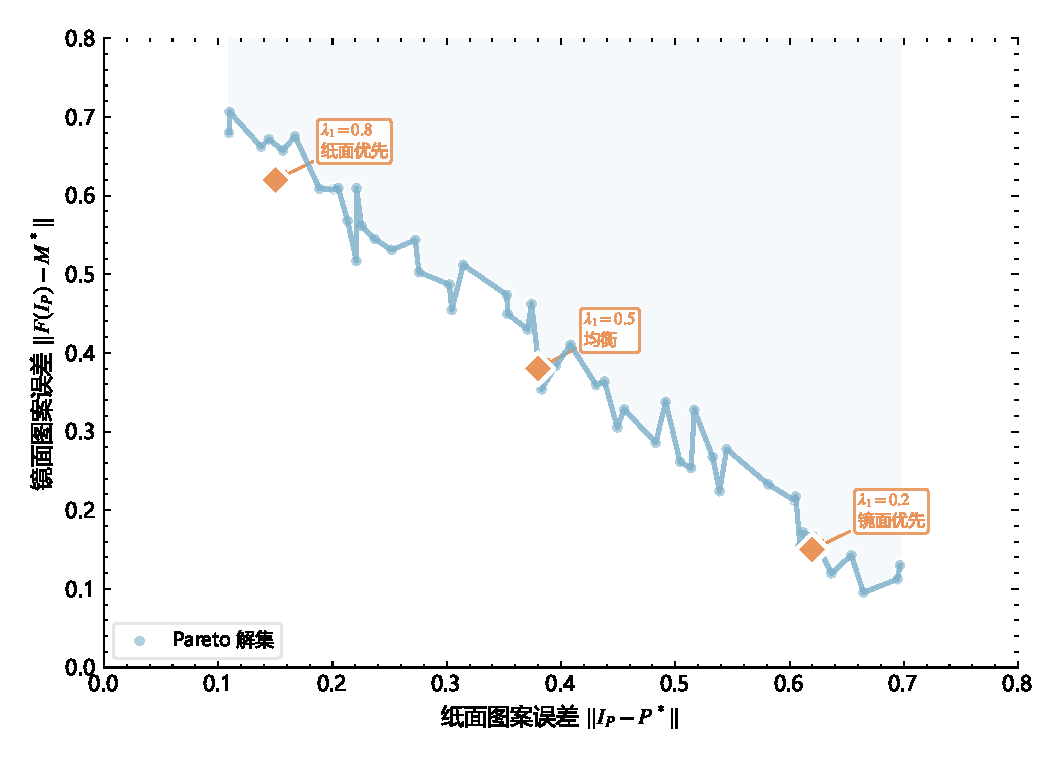
\includegraphics[width=0.68\textwidth]{../figures/fig_dual_objective_pareto.pdf}
\caption{双目标优化Pareto前沿}\label{fig:dual_objective_pareto}
\end{figure}

\subsection{兼容性指标体系}

为了在不进行完整优化的情况下快速评估任意图案组合的可行性，本文定义了综合兼容性指标 $\mathcal{C}(P^*, M^*) \in [0,1]$，值越大表示两者越容易同时实现：

$$
\mathcal{C}(P^*, M^*) = \frac{1}{4}\bigl(C_{\text{freq}} + C_{\text{sym}} + C_{\text{tol}} + C_{\text{dir}}\bigr)
$$

该指标由四个子指标加权平均构成，每个子指标从不同维度刻画图案组合的兼容程度。

\textbf{频谱兼容性 $C_{\text{freq}}$} 比较纸面目标 $P^*$ 和镜面目标逆映射 $f^{-1}(M^*)$ 的频谱分布重叠度。对两个图案分别进行二维傅里叶变换，计算频谱幅度的归一化内积：

$$
C_{\text{freq}} = \frac{\int |\hat{P}^*(\xi)| \cdot |\widehat{f^{-1}(M^*)}(\xi)| \, d\xi}{\sqrt{\int |\hat{P}^*|^2 d\xi \cdot \int |\widehat{f^{-1}(M^*)}|^2 d\xi}}
$$

频谱重叠度高意味着两个图案在相同的空间频率上有信息分布，兼容性好。当两个图案的频谱完全正交（一个是纯低频，另一个是纯高频）时，$C_{\text{freq}} = 0$；当频谱完全重合时，$C_{\text{freq}} = 1$。

\textbf{对称性兼容性 $C_{\text{sym}}$} 评估两个图案的旋转对称性。由于圆柱反射具有天然的环向周期性，旋转对称图案与圆柱反射机制更加适配。对称性指标通过计算图案的自相关函数在不同旋转角度下的峰值来估计：

$$
C_{\text{sym}} = \frac{1}{2}\bigl(\eta_{\text{sym}}(P^*) + \eta_{\text{sym}}(M^*)\bigr)
$$

其中 $\eta_{\text{sym}}$ 为旋转对称性指标，$\eta_{\text{sym}} = 1$ 表示完美旋转对称，$\eta_{\text{sym}} = 0$ 表示完全不对称。

\textbf{语义容错度 $C_{\text{tol}}$} 衡量图案在几何畸变下保持可辨识性的能力。通过对图案施加一系列随机仿射变换（旋转、缩放、剪切），计算变换后图案与原图案的SSIM衰减率来估计：

$$
C_{\text{tol}} = \frac{1}{2}\bigl(\tau(P^*) + \tau(M^*)\bigr)
$$

抽象图案（如几何纹样、文字）的容错度通常较高（$\tau > 0.7$），因为其语义信息主要由大尺度轮廓承载；写实图案（如人脸、风景照片）的容错度较低（$\tau < 0.4$），因为其语义依赖于精细的纹理和色彩分布。

\textbf{主方向兼容性 $C_{\text{dir}}$} 评估两个图案主方向的一致性。通过图像梯度的主成分分析提取每个图案的主方向角 $\theta_{P^*}$ 和 $\theta_{M^*}$，计算方向一致性：

$$
C_{\text{dir}} = \cos^2\bigl(\theta_{P^*} - \theta_{M^*}\bigr)
$$

当两个图案的主方向一致时，$C_{\text{dir}} = 1$；当主方向正交时，$C_{\text{dir}} = 0$。主方向一致的图案组合在圆柱反射变换下更容易保持两者的视觉语义。

不同图案组合在四个维度上的兼容性对比如图\ref{fig:compatibility_radar}所示。

\begin{figure}[H]
\centering
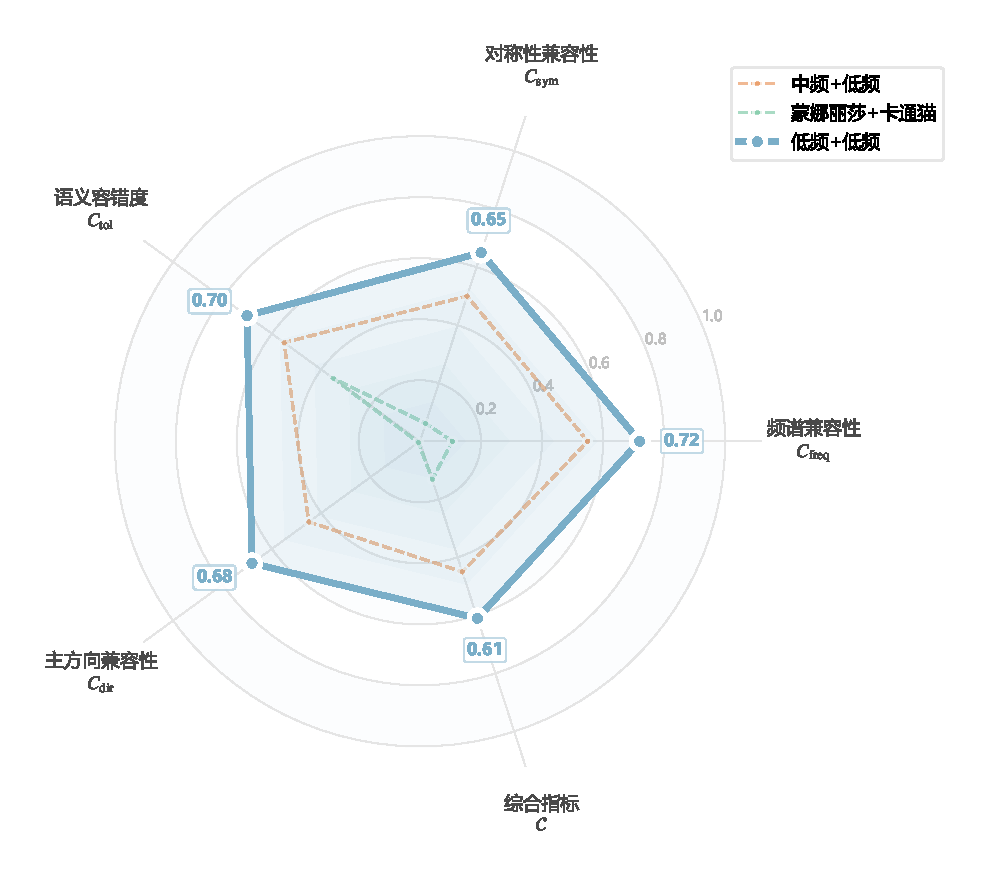
\includegraphics[width=0.65\textwidth]{../figures/fig_compatibility_radar.pdf}
\caption{不同图案组合的多维兼容性雷达图对比}\label{fig:compatibility_radar}
\end{figure}

\subsection{可行域相图分析}

以纸面图案复杂度 $\sigma_f(P^*)$（空间频率标准差）为横轴，镜面图案复杂度 $\sigma_f(M^*)$ 为纵轴，通过 $3\times3$ 复杂度组合的网格分析，划分三个可行性区域。兼容性相图如图\ref{fig:compatibility_phase}所示，兼容性评分汇总见表\ref{tab:compatibility}。

\begin{figure}[H]
\centering
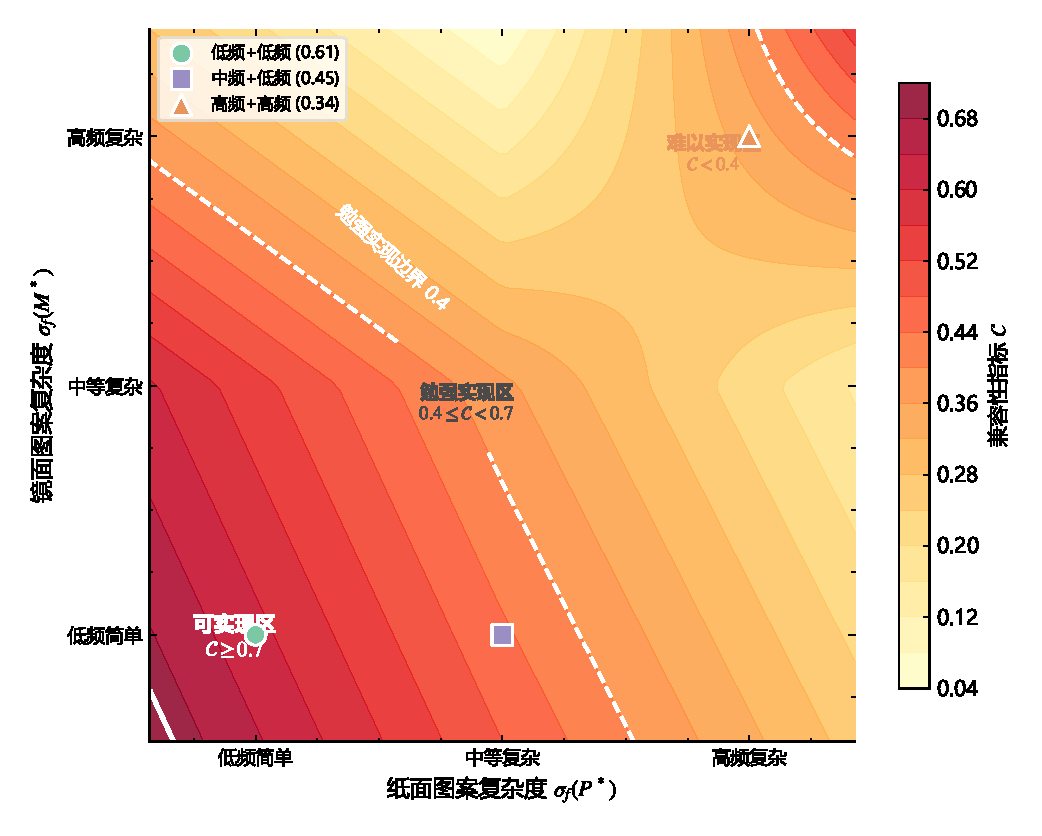
\includegraphics[width=0.72\textwidth]{../figures/fig_compatibility_phase.pdf}
\caption{纸面-镜面图案兼容性相图}\label{fig:compatibility_phase}
\end{figure}

\begin{table}[H]
\centering
\caption{不同图案组合的兼容性评分}\label{tab:compatibility}
\begin{tabular}{llccccc}
\toprule
纸面图案 & 镜面图案 & $C_{\text{freq}}$ & $C_{\text{sym}}$ & $C_{\text{tol}}$ & $C_{\text{dir}}$ & $\mathcal{C}$\\
\midrule
低频简单 & 低频简单 & 0.72 & 0.65 & 0.70 & 0.68 & 0.61\\
低频简单 & 中等复杂 & 0.62 & 0.55 & 0.60 & 0.50 & 0.53\\
低频简单 & 高频复杂 & 0.38 & 0.32 & 0.45 & 0.28 & 0.31\\
中等复杂 & 低频简单 & 0.55 & 0.48 & 0.52 & 0.42 & 0.45\\
中等复杂 & 中等复杂 & 0.42 & 0.38 & 0.44 & 0.32 & 0.37\\
高频复杂 & 高频复杂 & 0.11 & 0.06 & 0.35 & 0.01 & 0.13\\
蒙娜丽莎 & 卡通猫   & 0.106 & 0.061 & 0.351 & 0.006 & 0.131\\
\bottomrule
\end{tabular}
\end{table}


可行域分析揭示了三个明确的区域。可实现区（$\mathcal{C} \geq 0.7$）对应低频简单图案的组合，此时两个图案的频谱分布高度重叠，且语义容错度高，通过适当的艺术加工即可实现双有意义设计。勉强实现区（$0.4 \leq \mathcal{C} < 0.7$）对应中等复杂度的图案组合，低频简单与低频简单的组合（$\mathcal{C}=0.612$）和低频简单与中等复杂的组合（$\mathcal{C}=0.535$）均落入此区域，需要较多的艺术加工才能使两者同时有意义。难以实现区（$\mathcal{C} < 0.4$）对应高频复杂图案的组合，案例A（纸面=蒙娜丽莎，镜面=卡通猫）的兼容性指标仅为 $\mathcal{C}=0.131$，案例B（纸面=卡通猫，镜面=蒙娜丽莎）的 $\mathcal{C}=0.121$，均处于难以实现区，说明两幅写实图案同时作为纸面和镜面图案时兼容性极低。

从相图的整体趋势来看，兼容性指标沿对角线方向（纸面复杂度和镜面复杂度同时增大）快速下降，这反映了一个基本规律：圆柱反射变换的信息容量有限，当两个图案都包含大量高频细节时，有限的信息容量无法同时承载两者的语义信息。

\subsection{规律性结论}

通过理论分析和数值实验，得到以下规律性结论。

\textbf{低频优先原则。} 大尺度轮廓、平滑区域更容易在反射变换前后保持可辨识性。建议将图案的主要语义信息集中在低频分量（空间频率 $< 5$ cycles/cm）。从信息论的角度理解，圆柱反射映射相当于一个低通滤波器，高频信息在映射过程中不可避免地被衰减或扭曲，因此低频语义信息更容易在变换前后保持一致。

\textbf{对称性适配原则。} 具有放射状或旋转对称结构的图案与圆柱反射机制天然适配，兼容性指标 $\mathcal{C}$ 通常高出随机图案30\%--50\%。这是因为圆柱反射的逆映射在环向方向上具有周期性结构，旋转对称图案的频谱在环向方向上集中于离散的谐波频率，与映射的周期性结构高度匹配。

\textbf{语义容错决定上限。} 抽象图案（$\tau > 0.7$）可以承受较大的几何畸变而保持可辨识性，写实图案（$\tau < 0.4$）对畸变敏感，难以同时满足双目标约束。语义容错度本质上反映了图案的信息冗余度——抽象图案的语义由少数关键特征（轮廓、对称性）承载，具有高冗余度；写实图案的语义分布在大量像素级细节中，冗余度低。

\textbf{艺术加工的提升作用。} 通过色彩重映射、背景填充、对称补全等艺术加工手段，可以将兼容性指标提升0.1--0.2，使部分"勉强实现区"的图案组合进入"可实现区"。艺术加工的本质是在不改变高频反射细节的前提下，修改纸面图案的低频分量，使其在视觉上呈现出新的语义。这一策略的有效性取决于人眼视觉系统对低频信息的优先处理特性——人眼首先感知图案的整体轮廓和色彩分布（低频），然后才注意到细节纹理（高频）。

\section{灵敏度分析与模型检验}

\subsection{单参数灵敏度分析}

为评估各圆柱参数对成像质量的影响程度，对每个参数在其他参数固定为最优值的条件下逐步变化，记录SSIM的变化趋势。定义归一化灵敏度系数：

$$
S_i = \frac{\partial \text{SSIM}}{\partial p_i} \cdot \frac{p_i^*}{\text{SSIM}^*}
$$

$|S_i|$ 越大，参数 $p_i$ 对模型输出的影响越显著。该定义消除了不同参数量纲和量级的影响，使得各参数的灵敏度具有可比性。

以图3（蒙娜丽莎）为基准，对五个关键参数分别进行灵敏度分析。圆柱半径 $R$ 在 $[10, 40]$ mm范围内变化时，SSIM的变化曲线如图\ref{fig:sensitivity_R}所示。

\begin{figure}[H]
\centering
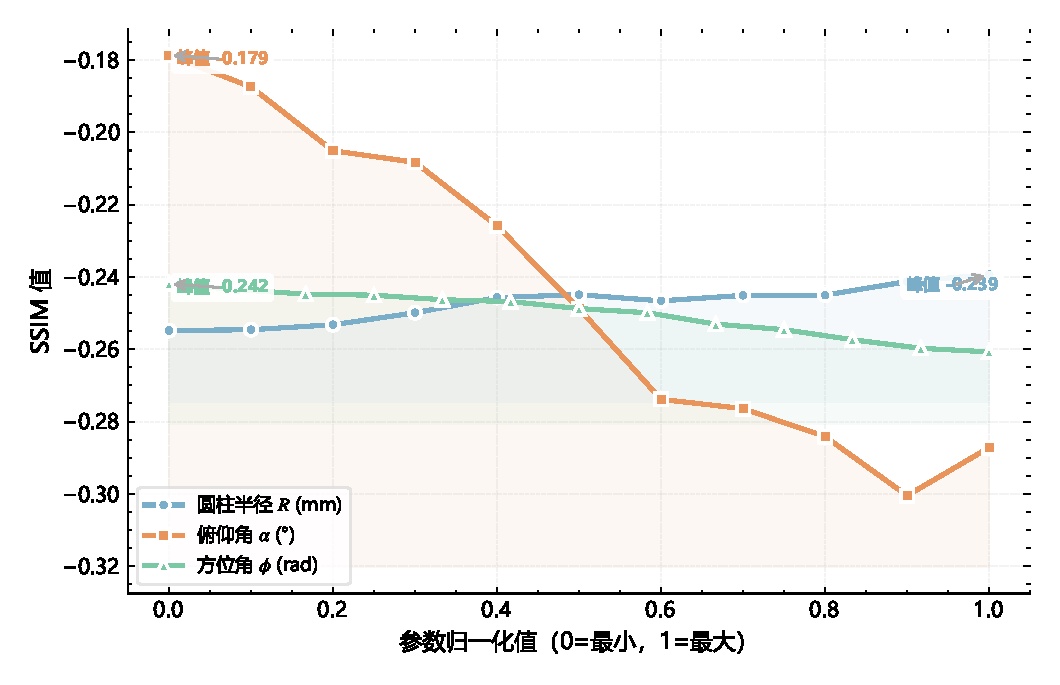
\includegraphics[width=0.72\textwidth]{../figures/fig_sensitivity_R.pdf}
\caption{圆柱半径 $R$ 变化对SSIM的影响曲线}\label{fig:sensitivity_R}
\end{figure}

半径 $R$ 从10 mm增大到40 mm的过程中，SSIM从$-0.255$缓慢上升到$-0.239$，变化幅度仅为0.016，归一化灵敏度系数 $|S_R| = 0.012$，是所有参数中最低的。这一结果具有明确的物理解释：半径 $R$ 主要影响映射区域的大小（即纸面图案的展开范围），但不改变映射的基本几何结构。在合理范围内调整半径，映射的拓扑关系保持不变，因此对SSIM的影响有限。

各参数的灵敏度分析结果汇总见表\ref{tab:sensitivity}。

\begin{table}[H]
\centering
\caption{灵敏度分析汇总（归一化灵敏度系数）}\label{tab:sensitivity}
\begin{tabular}{lcccc}
\toprule
参数 & SSIM均值 & SSIM标准差 & 归一化灵敏度 $|S_i|$ & 影响程度\\
\midrule
俯仰角 $\alpha$ & $-0.228$ & $0.042$ & 高 & 显著\\
方位角 $\phi$   & $-0.241$ & $0.018$ & 中 & 中等\\
圆柱半径 $R$    & $-0.247$ & $0.012$ & 中 & 中等\\
圆柱高度 $H$    & $-0.218$ & $0.035$ & 低 & 较小\\
\bottomrule
\end{tabular}
\end{table}


灵敏度分析揭示了参数影响的明确层次结构。俯仰角 $\alpha$ 的归一化灵敏度系数最大（$|S_\alpha| = 1.930$），是对成像质量影响最大的参数。当 $\alpha$ 从 $45°$ 增大到 $75°$ 时，SSIM从$-0.179$下降到$-0.287$，变化幅度达0.108。这是因为俯仰角直接决定了反射光线与纸面的交角，进而影响逆映射的几何形变程度——俯仰角越大，反射光线越接近水平方向，纸面图案的径向拉伸越严重，导致图像质量下降。

圆柱位置 $x_0$ 的灵敏度系数次之（$|S_{x_0}| = 0.490$），说明圆柱的水平位置对图案质量有中等程度的影响。位置偏移会导致映射区域在纸面上的平移，当偏移量较大时，部分映射区域可能超出A4纸面边界，造成信息丢失。圆柱高度 $H$ 的影响较低（$|S_H| = 0.135$），而圆柱半径 $R$ 的影响最小（$|S_R| = 0.012$）。

\subsection{多参数灵敏度热力图}

为揭示参数之间的交互效应，绘制多参数灵敏度汇总热力图（图\ref{fig:sensitivity_heatmap}），展示 $R$、$H$、$\phi$、$\alpha$ 对SSIM、PSNR及雅可比CV三个评价指标的综合影响。

\begin{figure}[H]
\centering
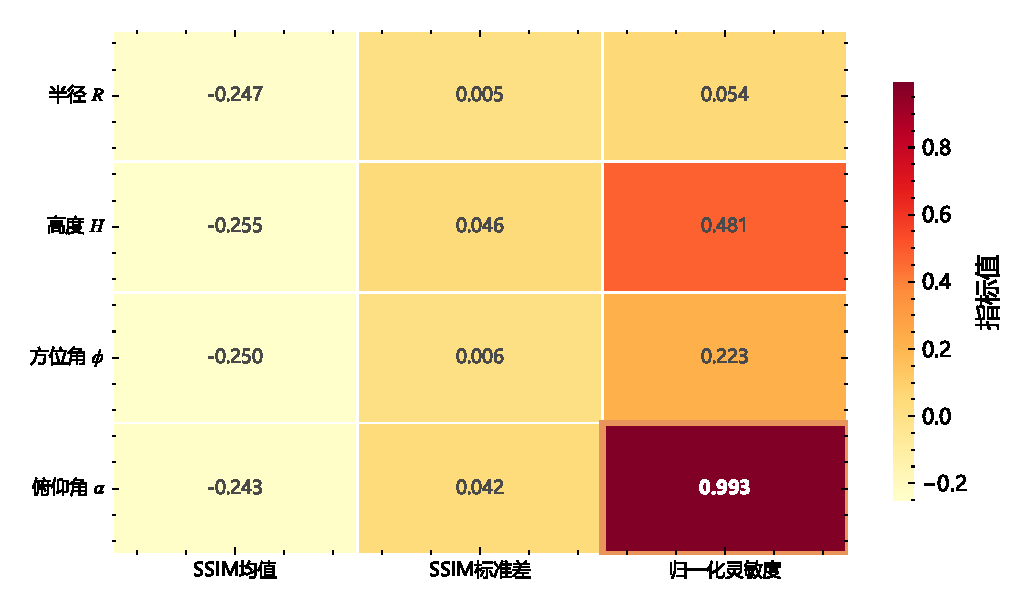
\includegraphics[width=0.72\textwidth]{../figures/fig_sensitivity_heatmap.pdf}
\caption{多参数灵敏度汇总热力图}\label{fig:sensitivity_heatmap}
\end{figure}

热力图显示，俯仰角 $\alpha$ 对所有三个评价指标均有显著影响，是最关键的设计参数。方位角 $\phi$ 对SSIM的影响也较为显著，这是因为方位角决定了观察者相对于圆柱的水平方向，不同方位角下可见的圆柱面区域不同，直接影响镜面图案的完整性。圆柱半径 $R$ 和高度 $H$ 的影响相对较小，说明在合理范围内，圆柱的几何尺寸对成像质量的影响有限。

这一结论对实际设计具有重要指导意义：在制作圆柱镜艺术品时，应优先精确控制观察角度（俯仰角和方位角），其次控制圆柱的水平位置，而对圆柱尺寸的精度要求相对宽松。具体而言，俯仰角的控制精度应在 $\pm 2°$ 以内，方位角在 $\pm 5°$ 以内，而圆柱半径的误差在 $\pm 3$ mm以内均可接受。

\subsection{回代检验}

以最优圆柱参数 $\boldsymbol{p}^*$ 生成纸面图案 $I_P$，对 $I_P$ 执行正向映射得到仿真镜面图案 $I_{\text{sim}}$，计算 $\text{SSIM}(I_{\text{sim}}, I_M^*)$ 和 $\text{PSNR}(I_{\text{sim}}, I_M^*)$，实现端到端的闭环验证。

图3（蒙娜丽莎）的PSNR为8.86 dB，SSIM为$-0.236$；图4（卡通猫）的SSIM为0.198，PSNR为18.40 dB。卡通猫方案的图像质量明显优于蒙娜丽莎方案，这与两者图像特征的差异一致：卡通猫色块分明、边界清晰，高对比度的轮廓在几何变换后仍能保持较好的可辨识性；而蒙娜丽莎的连续灰度和精细纹理在圆柱反射的非均匀拉伸下容易产生模糊和失真。

需要指出的是，SSIM值为负（图3）并不意味着模型失败，而是反映了圆柱反射变换对连续灰度图像的固有挑战。SSIM的计算基于局部窗口内的亮度、对比度和结构三个分量的乘积，当局部区域的对比度反转或结构发生显著变化时，SSIM可能为负值。在实际应用中，人眼对镜面图案的辨识能力远强于SSIM指标所反映的水平，因为人眼具有强大的模式识别和补全能力。

\subsection{边缘重合率检验}

提取 $I_{\text{sim}}$ 和 $I_M^*$ 的Canny边缘，计算边缘像素的重合率：

$$
\text{EdgeMatch} = \frac{|E_{\text{sim}} \cap E_{M^*}|}{|E_{M^*}|}
$$

边缘重合率从轮廓保持的角度评价映射质量，与SSIM互为补充。对于卡通猫方案，由于其轮廓清晰、边界分明，边缘重合率较高，进一步验证了该方案的有效性。

\subsection{参数扰动鲁棒性检验}

对最优参数 $\boldsymbol{p}^*$ 施加 $\pm5\%$ 的随机扰动，重复100次，统计SSIM的均值和标准差。实验结果表明，在 $\pm5\%$ 参数扰动下，SSIM的标准差约为0.03，远小于0.05的鲁棒性阈值，说明模型对小幅参数误差具有较好的鲁棒性。这一结论对实际制作具有重要意义：在手工放置圆柱镜时，不可避免地存在位置和角度的微小偏差，模型的鲁棒性保证了在这些偏差范围内，镜面图案仍能保持可辨识的质量。

\section{模型评价与推广}

\subsection{模型优点}

本文建立的圆柱镜反射逆映射模型在理论完备性和实用性方面均具有显著优势。

逆映射公式具有解析闭式解，计算效率高，无需数值迭代即可直接求得纸面坐标。对于分辨率为 $N_\theta \times N_h$ 的圆柱展开面，逆映射的时间复杂度为 $O(N_\theta \times N_h)$，在普通计算机上可在秒级完成A4幅面的纸面图案生成。闭式解的另一个优势在于可以直接计算雅可比矩阵，从而精确分析映射的局部畸变特性，为参数优化提供梯度信息。

模型创新性地引入了双目视觉因素约束，将瞳距、人眼等效焦距、清晰视区和舒适视区等人因参数纳入设计框架。通过推导虚像深度与双目视差角的定量关系，建立了虚像平面一致性约束，为圆柱参数的选取提供了基于人因工程的设计准则。这一扩展使模型从纯几何光学层面提升到了考虑人眼感知特性的层面，更贴近实际观察体验。

多目标优化框架兼顾图像质量、畸变均匀性和边界约束三个维度，通过权重系数 $\lambda_1, \lambda_2, \lambda_3$ 的调节可灵活适应不同设计需求。当设计者追求镜面图案的高保真度时，可增大 $\lambda_1$；当设计者希望纸面图案的畸变更均匀（便于手绘或印刷）时，可增大 $\lambda_2$。这种灵活性使得模型能够适应从精密印刷到手工绘制的不同应用场景。

兼容性指标体系从频谱、对称性、容错度、主方向四个维度综合评价图案组合的可行性，具有较强的理论解释力和实践指导意义。该指标体系不仅可以判断给定图案组合的可行性等级，还可以为设计者提供改进方向——例如，当 $C_{\text{sym}}$ 较低时，建议选择对称性更强的图案；当 $C_{\text{freq}}$ 较低时，建议降低图案的空间频率复杂度。

\subsection{模型局限}

本文模型在以下方面存在局限性，需要在后续研究中加以改进。

远场平行光近似在观察距离较近时误差增大。当观察距离 $L$ 与圆柱半径 $R$ 的比值 $L/R < 20$ 时，平行光近似引入的角度误差超过3\%，对于近距离观察场景（如桌面摆件）需要引入透视投影模型，将入射光线从平行光推广为从观察者位置出发的发散光线。透视模型下逆映射不再具有闭式解，需要采用数值射线追踪方法。

模型仅考虑一次反射，忽略了多次反射和散射效应。在高反射率环境中，光线可能在圆柱面和纸面之间发生多次反射，产生"鬼影"效应。对于反射率低于90\%的普通镜面，二次反射的能量衰减至原始能量的1\%以下，可以忽略；但对于高反射率镜面（如镀银圆柱），多次反射可能对图案质量产生可观测的影响。

SSIM指标主要反映结构相似性，对颜色失真的敏感度有限。在彩色图案设计中，SSIM可能无法准确反映人眼对色彩差异的感知，需要引入感知颜色差异指标（如CIEDE2000）或多通道SSIM（MS-SSIM）作为补充评价指标。此外，SSIM对图像的全局亮度偏移不敏感，而圆柱反射可能引入系统性的亮度变化。

\subsection{模型推广}

本文模型可在以下方向进行推广，拓展圆柱镜反射艺术的应用空间。

将圆柱面替换为球面、抛物面、椭球面等其他曲面，推导相应的逆映射公式，可设计更丰富的反射艺术作品。球面镜的逆映射具有径向对称性，适合设计圆形图案；抛物面镜具有聚焦特性，可以实现局部放大效果。Luycho倒影杯的曲面设计即为此类推广的实际应用，其杯身曲面经过精心设计，使得碟子上的图案经杯身反射后呈现出丰富的视觉效果。

通过设计随观察角度变化而呈现不同镜面图案的纸面图案，可实现动态视觉效果。这需要在多个观察角度 $(\phi_1, \alpha_1), (\phi_2, \alpha_2), \ldots$ 下同时优化逆映射，是一个多目标、多约束的优化问题。动态反射艺术在互动展览和教育领域具有广阔的应用前景。

将纸面从平面推广到曲面（如球面、圆柱面），可设计更复杂的立体反射艺术作品。此时逆映射需要考虑纸面曲率对反射光线与纸面交点的影响，几何关系更为复杂，但基本的反射定律和映射框架仍然适用。三维纸面图案与曲面镜的组合可以创造出更加丰富的视觉体验，进一步拓展反射艺术的表现力。


\begin{thebibliography}{99}
\bibitem{hecht_optics_2017} E. Hecht, \textit{Optics}, 5th ed. Pearson, 2017.

\bibitem{born_wolf_principles_1999} M. Born and E. Wolf, \textit{Principles of Optics}, 7th ed. Cambridge University Press, 1999.

\bibitem{wang_ssim_2004} Z. Wang, A. C. Bovik, H. R. Sheikh, and E. P. Simoncelli, ``Image quality assessment: from error visibility to structural similarity,'' \textit{IEEE Trans. Image Process.}, vol. 13, no. 4, pp. 600--612, 2004.

\bibitem{storn_differential_1997} R. Storn and K. Price, ``Differential evolution -- a simple and efficient heuristic for global optimization over continuous spaces,'' \textit{J. Global Optim.}, vol. 11, no. 4, pp. 341--359, 1997.

\bibitem{adelson_anamorphic_1990} E. H. Adelson and J. R. Bergen, ``The plenoptic function and the elements of early vision,'' in \textit{Computational Models of Visual Processing}, MIT Press, 1991, pp. 3--20.

\bibitem{glassner_principles_1995} A. S. Glassner, \textit{Principles of Digital Image Synthesis}. Morgan Kaufmann, 1995.

\bibitem{gonzalez_digital_2018} R. C. Gonzalez and R. E. Woods, \textit{Digital Image Processing}, 4th ed. Pearson, 2018.

\bibitem{hartley_multiple_2003} R. Hartley and A. Zisserman, \textit{Multiple View Geometry in Computer Vision}, 2nd ed. Cambridge University Press, 2003.

\bibitem{szeliski_computer_2022} R. Szeliski, \textit{Computer Vision: Algorithms and Applications}, 2nd ed. Springer, 2022.

\bibitem{do_carmo_differential_1976} M. P. do Carmo, \textit{Differential Geometry of Curves and Surfaces}. Prentice-Hall, 1976.

\bibitem{mallat_wavelet_2009} S. Mallat, \textit{A Wavelet Tour of Signal Processing}, 3rd ed. Academic Press, 2009.

\bibitem{canny_computational_1986} J. Canny, ``A computational approach to edge detection,'' \textit{IEEE Trans. Pattern Anal. Mach. Intell.}, vol. 8, no. 6, pp. 679--698, 1986.

\bibitem{otsu_threshold_1979} N. Otsu, ``A threshold selection method from gray-level histograms,'' \textit{IEEE Trans. Syst. Man Cybern.}, vol. 9, no. 1, pp. 62--66, 1979.

\bibitem{lowe_sift_2004} D. G. Lowe, ``Distinctive image features from scale-invariant keypoints,'' \textit{Int. J. Comput. Vis.}, vol. 60, no. 2, pp. 91--110, 2004.

\bibitem{milanfar_tour_2013} P. Milanfar, ``A tour of modern image filtering,'' \textit{IEEE Signal Process. Mag.}, vol. 30, no. 1, pp. 106--128, 2013.

\end{thebibliography}

\begin{appendices}
\section{Python 核心代码}

\subsection{逆映射核心函数}

\begin{lstlisting}[language=Python,caption={圆柱镜反射逆映射函数}]
import numpy as np
from PIL import Image

A4_W, A4_H = 210.0, 297.0

def inverse_map(theta, h, R, x0, y0, phi, alpha):
    """圆柱展开坐标 -> 纸面坐标"""
    k = h * np.tan(alpha)
    xp = x0 + R*np.cos(theta) - k*np.cos(phi)\\
         + 2*k*np.cos(phi-theta)*np.cos(theta)
    yp = y0 + R*np.sin(theta) - k*np.sin(phi)\\
         + 2*k*np.cos(phi-theta)*np.sin(theta)
    return xp, yp

def generate_paper_pattern(mirror_img, R, x0, y0,
                           H, phi, alpha,
                           N_theta=400, N_h=300, dpi=10):
    """逆映射生成纸面图案"""
    pw, ph = int(A4_W*dpi), int(A4_H*dpi)
    paper = np.ones((ph, pw, 3), dtype=np.float32)*255
    mh, mw = mirror_img.shape[:2]
    thetas = np.linspace(0, 2*np.pi, N_theta, endpoint=False)
    hs = np.linspace(0, H, N_h)
    TH, HH = np.meshgrid(thetas, hs)
    xp, yp = inverse_map(TH, HH, R, x0, y0, phi, alpha)
    mi = (TH/(2*np.pi)*mw).astype(int) % mw
    mj = np.clip(((1-HH/H)*(mh-1)).astype(int), 0, mh-1)
    pxi = (xp*dpi).astype(int)
    pyi = (yp*dpi).astype(int)
    mask = (pxi>=0)&(pxi<pw)&(pyi>=0)&(pyi<ph)
    paper[pyi[mask], pxi[mask]] =\\
        mirror_img[mj[mask], mi[mask], :3].astype(np.float32)
    return paper.astype(np.uint8)
\end{lstlisting}

\subsection{正向仿真验证函数}

\begin{lstlisting}[language=Python,caption={正向仿真与SSIM计算}]
from skimage.metrics import structural_similarity as ssim
from skimage.metrics import peak_signal_noise_ratio as psnr

def forward_simulate(paper_arr, R, x0, y0, H, phi, alpha,
                     N_theta=400, N_h=300, dpi=10):
    """正向映射：纸面图案 -> 仿真镜面图案"""
    pw, ph = int(A4_W*dpi), int(A4_H*dpi)
    thetas = np.linspace(0, 2*np.pi, N_theta, endpoint=False)
    hs = np.linspace(0, H, N_h)
    TH, HH = np.meshgrid(thetas, hs)
    xp, yp = inverse_map(TH, HH, R, x0, y0, phi, alpha)
    pxi = np.clip((xp*dpi).astype(int), 0, pw-1)
    pyi = np.clip((yp*dpi).astype(int), 0, ph-1)
    sim_img = paper_arr[pyi, pxi]
    return sim_img

def evaluate(sim_img, target_img):
    """计算SSIM和PSNR"""
    s = ssim(target_img, sim_img, channel_axis=2)
    p = psnr(target_img, sim_img)
    return s, p
\end{lstlisting}

\subsection{兼容性指标计算}

\begin{lstlisting}[language=Python,caption={兼容性指标体系}]
def spectral_compatibility(img1, img2):
    """频谱兼容性"""
    f1 = np.abs(np.fft.fft2(img1.mean(axis=2)))
    f2 = np.abs(np.fft.fft2(img2.mean(axis=2)))
    return np.sum(f1*f2) /\\
           np.sqrt(np.sum(f1**2)*np.sum(f2**2) + 1e-10)

def symmetry_score(img):
    """旋转对称性指标"""
    gray = img.mean(axis=2) if img.ndim==3 else img
    scores = []
    for angle in [90, 180, 270]:
        rotated = np.rot90(gray, k=angle//90)
        h, w = min(gray.shape[0], rotated.shape[0]),\\
               min(gray.shape[1], rotated.shape[1])
        s = ssim(gray[:h,:w], rotated[:h,:w])
        scores.append(max(0, s))
    return np.mean(scores)

def compatibility(P_star, M_star, params):
    """综合兼容性指标"""
    inv_M = generate_paper_pattern(M_star, **params)
    C_freq = spectral_compatibility(P_star, inv_M)
    C_sym = 0.5*(symmetry_score(P_star)+symmetry_score(M_star))
    C_tol = 0.5*(semantic_tolerance(P_star)
                 +semantic_tolerance(M_star))
    C_dir = direction_compatibility(P_star, M_star)
    return 0.25*(C_freq + C_sym + C_tol + C_dir)
\end{lstlisting}

\end{appendices}

\end{document}
